\pdfoutput=1

\RequirePackage{fix-cm}
\RequirePackage{rotating}

\documentclass[smallextended]{svjour3}
\smartqed 
% \usepackage[5]{lineno}
% \linenumbers
\usepackage{cite}
\usepackage{mathptmx}
\usepackage{rotate}
\usepackage{amsmath,amssymb,amsfonts}
\usepackage{algorithmic}
\usepackage{graphicx}
\usepackage{subcaption}
\captionsetup{compatibility=false}
\usepackage{textcomp}
\usepackage{xcolor}
\usepackage{listings}
\usepackage{multirow}
\usepackage{xcolor,colortbl}
\usepackage[flushleft]{threeparttable}
\usepackage{amsmath}
\usepackage{relsize}
\usepackage{pifont}
\usepackage{wrapfig}
\usepackage{url}
\usepackage[sort&compress,numbers]{natbib}
\usepackage[bottom]{footmisc}
% \feetbelowfloat

\usepackage{wasysym}
% \usepackage{unicode-math}

\usepackage{pgfplots}

\usepackage{changepage} 

\pgfplotsset{compat=1.10}
\usepgfplotslibrary{fillbetween}

\def\BibTeX{{\rm B\kern-.05em{\sc i\kern-.025em b}\kern-.08em
    T\kern-.1667em\lower.7ex\hbox{E}\kern-.125emX}}
    
\definecolor{MyDarkBlue}{rgb}{0,0.08,0.45} 
\lstset{
    language=Python,
    basicstyle=\sffamily\fontsize{2.5mm}{0.7em}\selectfont,
    breaklines=true,
    prebreak=\raisebox{0ex}[0ex][0ex]{\ensuremath{\hookleftarrow}},
    frame=l,
    keepspaces=false,
    showtabs=false,
    columns=fullflexible,
    showspaces=false,
    showstringspaces=false,
    keywordstyle=\bfseries\sffamily,
    emph={ m, r, k, frontier, cf, f, g, n, tData, nrefs, cMax, inertia, gaps,trainData, testData, Word2Vec_model, trainX, trainY, cluster, svm_models, totalDlusterY,predictedC, r, threads, predicted, data, predict,cluster_model , classification_model}, emphstyle=\bfseries\color{blue!50!black},
    stringstyle=\color{green!50!black},
    commentstyle=\color{red!50!black}\it,
    numbers=left,
    captionpos=t,
    escapeinside={\%}{)}
}
    


\usepackage{pifont}
\usepackage{listings}
\usepackage{tcolorbox}
\newtcolorbox{blockquote}{colback=red!5!white,boxrule=0.4pt,colframe=red!50!black,fonttitle=\bfseries,top=2pt,bottom=2pt}

\newcommand{\bi}{\begin{itemize}}
\newcommand{\ei}{\end{itemize}}

\usepackage{tabularx}
\usepackage{multirow}
\usepackage{color,colortbl}
\definecolor{lightgray}{gray}{0.8}
\usepackage{adjustbox}

\usepackage{amssymb}% http://ctan.org/pkg/amssymb
\usepackage{pifont}% http://ctan.org/pkg/pifont
\newcommand{\cmark}{\ding{51}}%
 


\newcommand{\tion}[1]{\S\ref{tion:#1}}

\newcommand{\fig}[1]{Figure~\ref{fig:#1}}

\newcommand{\tbl}[1]{Table~\ref{tbl:#1}}

%%%%%%%%%%%%%%%%%%%%%%%%%%%%%%%%%%%%%%%%%%%%%%%%%%

% %%%%%%%%%%%%
\newcommand{\citeresp}[1]{%
{(please see }\fcolorbox{black}{black!15}{%
\bf\scriptsize R{#1}}~{{on page \pageref{resp:#1})}}}%

\newcommand{\respto}[1]{
\fcolorbox{black}{black!15}{%
\label{resp:#1}%
\bf\scriptsize R{#1}}}

\newcommand{\MARK}{\color{blue}}
% %%%%%%%%%%%%%
\newcommand{\review}[1]{{\textit{#1}}~\\}
\newcommand{\revised}{\textcolor{blue}}
%%%%%%%%%%%%%%%%%%%%%%%%%%%%%%%%%%%%%%%%%%%%%%%%
\newcommand{\quart}[4]{
\begin{picture}(100,6)%1
    {
        \color{black}
        \put(#3,3)
        {\circle*{4}}
        \put(#1,3)
        {\line(1,0){#2}}
    }
\end{picture}
}


\newcommand{\BLUE}{\color{blue}}
\newcommand{\BLACK}{\color{black}}
\newcommand{\RED}{\color{red}}


\begin{document}

\textbf{EMSE Major Revision Round 2}

\bigskip
\section*{Response to Editor}


\BLUE
We  want to thank all reviewers (especially Reviewer 4) for their careful and insightful comments. Typos are fixed  and readability is improved with careful proof-reading. According to reviewers' comments, we have revised the draft  (shown as \respto{1}, \respto{2} and \respto{4}, respectively).

\bigskip

\BLACK
{\em ``We will make an accept/reject decision based on the next revision. ''}

\bigskip

\BLUE
We appreciate the second opportunity to revise this paper. We also understand the above point since
it does not make sense to have papers stuck in endless revision cycles. 
However, since 
\bi
\item
We have seen a new reviewer (Reviewer 4) this round; and
\item
That reviewer has added several new added requirements not seen in the prior reviewers' requests
\ei
we want to ask, would it be possible to have more chances for the revisions?
We ask this since,
while we are trying our best to respond to those new comments, it would be very appreciated if more opportunities are granted to improve the current manuscript.


\BLACK

\bigskip


\section*{Response to Reviewer \#1}

\review{\textbf{Round2-R1-A:} I would prefer the author reply regarding task bias (regarding parameters from literature) to have a footprint in the manuscript.
}

\BLUE
Thanks for the comments. We have added a footnote to explain the parameters using in Model Construction section. \citeresp{1A}
\BLACK
\bigskip

\review{\textbf{Round2-R1-B:} It could benefit from minor copy-edits which I list below; however, most are suggestions rather than corrections.
}

\BLUE
Thanks for the suggestions, we have edited and polished the corresponding words and fixed typos as well.
\BLACK
\bigskip


% You also write \BLACK Crucially, combined with an  analysis of the importance of different features for the machine learning models,which would in turn improve our understanding of what affects the health of a project,with time periods that have an effect.

% \bigskip

% \RED
% Here, we must report a negative result.
% We can find no general pattern in what features seem most important in this data:
% \bi
% \item
% In the last draft we showed that using a method that counted how often variables appeared in the learned regression trees.  
% \item
% You, and other reviewers,  objected to our home-brew feature importance methods. So rather than invent a new one (with no precedent),   we decided to use  a method that was more standard.
% \item So we went to scikit-learn and looked
% for their standard methods to evaluate the importance of the features.
% \item That took
% us to the new tree-based method used in this paper. The Gini importance
% algorithm  computes  impurity-based feature importances
% (.e.g the importance of a feature is computed as the normalized total reduction of the criterion brought by the feature).  \citeresp{4F}
% \ei
% The key point to note here is that according to {\em both} our feature importance studies (the Gini-based analysis in this draft AND the tree membership method used in the last draft), there is no clear pattern in what features are most important (see Table~\ref{tbl:frq}). This is clearly a matter for future work.
% \BLACK


 
\newpage
\section*{Response to Reviewer \#2}


\review{\textbf{Round2-R2-A:} I am not convinced by the answer given to comment R1c. Since the authors indicated to have used FLASH for parameter tuning in the previous version of the manuscript, why not reporting the results? Or why not directly report that FLASH does not always work as believed and written by the same authors of this manuscript in prior studies?
}

\BLUE
Thanks for the comments. Initially we were trying to prove that hyperparameter tuning can improve the prediction performance in our experiments. We tested a few optimizers and selected DE in the first manuscript. With your suggestion, we have added method tuned by FLASH in our benchmarks, updated the experiments results and reported that FLASH does not always work the best in the experiments. \citeresp{2A1} \citeresp{2A2}
\BLACK
\bigskip

\review{\textbf{Round2-R2-B:} GSCART (grid search) is much slower than DECART. This is true only if using a different number of trials/samples. Keeping the same number of trial configurations N, DECART requires by definition more running time due to the complexity of the evolutionary operator. Instead, grid search tries N configuration with no additional operators. How do DECART and GSCAR when using the same number of trials/samples?
}


\BLUE
We agree with you on this that we made an unfair comparison between GSCART and DECART in the previous manuscript. To fix this issue, we have set the budget of GSCART (grid search) the same number of trials as other optimizers (e.g. DECART), re-run the experiments on whole dataset and updated the results. \citeresp{2B}
\BLACK
\bigskip

\review{\textbf{Round2-R2-C:} The authors used the non-parametric variant of the Scott-Knott statistical test introduced by Mittas et al. in TSE'13. However, as pointed out by H. Steffen, the correction made by Mittas et al. to this test "does not necessarily lead to the fulfillment of the assumptions of the original Scott-Knott test and may cause problems with the statistical analysis." Long story short, Scott-Knott is not a correct statistical test for non-normally distributed data. I strongly recommend using either the ANOVA (with permutation) or the Friedman tests instead. Suppose the authors insist on using the Scott-Knott statistical test. In that case, they MUST provide theoretical evidence that the concerns raised by H. Steffen do not hold in this case.
}


\BLUE
Thanks for the suggestions. We have replaced the Scott-Knott statistical test by Friedman test with Nemenyi Post-Hoc test. In this new manuscript, for each project, we first use Friedman test to determine if there are statistical significant differences between the performance of predictors. If yes, we then use Nemenyi post-hoc test to determine which predictor(s) are statistically better. \citeresp{2C}
\BLACK
\bigskip


\review{\textbf{Round2-R2-D:} I'm afraid I have to disagree with the argument "Many feature selection mechanisms are somewhat arcane and, hence, make it hard to explaining to business users." This argument in the response letter is problematic in two ways:
Arcane does not imply bad. If we go for that route, one can argue that the Turing machine is "bad" because it is 70+ years old. Of course, that is not the case.
Many existing feature selection methods are straightforward to explain and apply. See, for example, unsupervised approaches based on simple correlation (to remove collinearity)
My recommendation to use well-established feature selection methods remains unless the authors provide better arguments than those used in the current response letter.
}



\BLUE
Thanks for the comments. We agree that it will be more convincing if we could use well-established methods for feature importance analysis. In this round,  we did some literature review and
found that tree-based method is one way that widely used. To fix the problem, we applied the tree-based method from scikit-learn and  evaluate the Gini importance of the features.
The Gini importance algorithm  computes  impurity-based feature importances
(the importance of a feature is computed as the normalized total reduction of the criterion brought by the feature).  \citeresp{2D}
\BLACK
\bigskip


\review{\textbf{Round2-R2-E:} Based on the survey results, the  "stargazers" indicator is marked as "irrelevant" by the majority of the participants (52\%). Why then keeping this indicator? This indicator should be removed to be consistent with the results of the developers' interviews.
}


\BLUE
Thanks for the suggestions. We have removed the stargazers prediction in the new experiments. \citeresp{2E}
\BLACK
 \bigskip

\review{\textbf{Round2-R2-F:} The text added to answer the comment Rx2f should be revisited: lines 23-35 describe another work by the authors of this manuscript that is entirely unrelated. Unnecessary self-citations should be avoided: there is no need to sell unrelated work.
On the other hand, the section does not provide a more compelling view of hyper-parameter optimization done in closely related fields. For example, evolutionary algorithms have been used in defect prediction or effort estimation to fine-tune the parameters of the same classifiers applied in this work (e.g., CART or J48 parameter tuning).
}

 
\BLUE
Thanks for the comments. We have removed the unrelated text and added more recent works of hyperparameter optimization in defect prediction, systems configuration and effort estimation. \citeresp{2F}
\BLACK
 \bigskip

\review{\textbf{Round2-R2-G:} The arguments justifying the usage of DE are unsatisfactory and mathematically incorrect (lines 24-38 on page 9). This paragraph is problematic for many reasons.
Reason 1: DE is one of the many evolutionary algorithms in the literature. It is not the most recent nor the best performing in all contexts (as this manuscript wants us to believe).
DE has indeed been shown to perform well on specific optimization problems. But it has also been shown to underperform on other optimization problems (e.g., non-linearly separable problem). I highly recommend the authors to look at Section VIII of the following survey:
[2] S. Das and P. N. Suganthan, "Differential Evolution: A Survey of the State-of-the-Art," in IEEE Transactions on Evolutionary Computation, vol. 15, no. 1, pp. 4-31, Feb. 2011, DOI: 10.1109/TEVC.2010.2059031.
Reason 2: I assume the authors are well familiar with the no-free lunch theorem. Hence, no algorithm is superior to all other algorithms on all optimization problems. This applies to DE and but also to different approaches (e.g., FLASH) the authors have proposed lately.
"We found that DE works just as well as anything else, ran much faster [...]." Compared to what? In absolute terms? For all problems? This statement is mathematically incorrect (see the no-free lunch theorem) but also empirically inaccurate as the authors did not compare DE to "anything else" in this work.
My final question, therefore, is: why not comparing DECART to other simpler evolutionary algorithms? If the authors insist on proposing DE as the best out there, they have to show that this is the case.
The only argument the authors can use is that the DE has shown good performance regarding grid search and random search. Analysis of other evolutionary algorithms (probably even better than DE) can be part of future work. Finally, the authors should not claim that DE "is the best" but simply better than the two baselines used in the study.
}

 
\BLUE
Thanks for pointing out the inappropriate description of DE in our last draft, we have revised the paragraph to describe the power of DE objectively. In this new draft, we want to indicate that DE gets good performance compared to other methods in our experiment, and we would explore other evolutionary algorithms for further improvement in the future work. \citeresp{2G1} \citeresp{2G2} \citeresp{2G3} \citeresp{2G4} \citeresp{2G5}
\BLACK
 \bigskip

\review{\textbf{Round2-R2-H:} I highly appreciate that the authors improved Table six addressing the comments Rx1f1 Rx2h. However, the table might still include one word that should not be excluded: "CV." If CV stands for "cross-validation," then it should not be included in the blocklist.
}


 
\BLUE
Thanks for the suggestion. We have removed ``CV'' from the blocklist. \citeresp{2H}
\BLACK
\bigskip

\review{\textbf{Round2-R2-I:} The authors should enrich the analysis of the results: In how many cases/projects are the results of DECART statistically better than those produced by the baselines? Are the percentages reported in Section 4.3 based on the number of statistically significant cases? Or based on whether the median/mean is larger?
}

 
\BLUE
Thanks for the comments. With the new experiment and statistical methods (Friedman test and Nemenyi test), we have updated our experiment results and performance evaluations. The percentages reported in Section 4.3 are based on the method's numbers of ``Rank=1'' appears in all cases. ``Rank=1'' means that the related method is in statistically the best performance group (the group may have multiple methods if they don't have statistically significant difference).
\citeresp{2I}
\BLACK
 

 
\clearpage

\section*{Response to Reviewer \#4}

\BLUE
Thank you for your detailed suggestions. For simplicity's sake, we have divided our replies to you into two parts.
  
  Firstly, we list all the changes we made resulting from your specific individual comments.
  
  Next, in  Round2-R4-I, we offer a combined analysis of several of your comments which, to our reading,
  were  aspects on one composite  meta-issue.
 \BLACK
\bigskip

\review{\textbf{Round2-R4-A:} 
Table 1 shows a mapping between the proposed features and Linux Kernel Practices, but how this mapping was determined was unclear to me... As far as I can tell, a mapping that maps everything to everything would be equally valid.
}


\BLUE
You are quite correct. We realize that the added
value of this table is not so much.
With your suggestion, we have removed it from this new manuscript and added related content to the introduction \citeresp{4A}.
\BLACK
\bigskip


\review{\textbf{Round2-R4-B:} 
The survey questions posed to the open source developers should be reported. In particular, it is unclear whether participants were given the task of rating the given properties or a more free-form survey where they were able to propose their own properties. The former would presumably introduce some bias ("choose the best from this menu of options").
}


\BLUE
Thanks for the comments. We have added the details of our survey questions. \citeresp{4B1} Regarding to the bias on ``choose the best from given'', we did give participants space to talk about their own opinions on additional health indicators if they have (Please see Question 4 in the survey). We also have added discussions about the bias in the section of Threats to validity, \citeresp{4B2} and future work about exploring more health indicators based on developers' opinions.   \citeresp{4B3}
\BLACK
\bigskip



\review{\textbf{Round2-R4-C:} 
(My main concern with the evaluation is that) the authors are modeling and learning time-series data, but only evaluating at a few chosen points in time. A standard approach to evaluating these kinds of models in the machine learning literature is to apply a moving window, where models are trained on
e.g. 6 months of data evaluated for the next month, then moved one month forward and evaluated again, and so on. This gives a much better picture of the reliability of the models and predictions at various points in time. This would also remove the need for repositories to be filtered by specific dates.
}



\BLUE
Thanks for the comments. We have re-designed the model training process and re-run the experiments. We took your suggestions and applied a ``sliding-window-style'' way to build the models training and testing pipeline.  \citeresp{4C} 
\BLACK
\bigskip

\review{\textbf{Round2-R4-D:} In addition to the summary results across all considered projects, a case study would be insightful. An error of 10\% is still relatively high, in particular if the numbers are used for project planning -- 110 pull requests require more work
and personnel than 100. The Linux kernel could be considered (I assume that it was included) to show how some of the prediction scenarios the authors outline at the beginning of the paper would play out (e.g. for personnel planning).
}


\BLUE
Thanks for the suggestions. We have added a real-world use case to show how our methods can be used (predicting number of contributors next month for a set of open source OS projects). 
\citeresp{4D} 
\BLACK
\bigskip

\review{\textbf{Round2-R4-E:} In the construction of the models, why is only 80\% of available data selected for training?
}


\BLUE
Thanks for the comments. In previous manuscript, we used 80\% of data for training to test the reliability and performance variability of the models. In this new manuscript, since the model training process and performance evaluation methods have been changed, we have removed this rule when training the model. \citeresp{4E1} \citeresp{4E2} 
\BLACK
\bigskip

\review{\textbf{Round2-R4-F:} The analysis of feature importance in section 4.2 should take the position of a feature split in the learned tree into account -- a feature that is used high up in the tree is much more important than a feature far down that only helps to discriminate between a small number of data points.
}


\BLUE
Thanks for the comments. With your permission, we wish to follow the spirit of your suggestion and replace the previous analysis method with something more standard.
To that end, we applied the tree-based method from scikit-learn and  evaluate the Gini importance of the features.
The Gini importance algorithm  computes  impurity-based feature importances
(the importance of a feature is computed as the normalized total reduction of the criterion brought by the feature). \citeresp{4F}
\BLACK
\bigskip



    

% \bigskip
% \RED
% Thanks for the comments. 
% Here again, like R4a,
% you are raising point that (to quote Shakespeare) 
% ``There are more things in heaven and Earth, Horatio, / Than are dreamt of in your philosophy''.
% We concur
% but we want to point that one of our objectives in this study is to see whether these straightforward GitHub features can affect the open source project as health indicators. Using these easy to access features instead of some very complex indexes is convenient and direct to get useful information about the health status of a project. 
% ~\\
% But, as we said in R4a, your general point remains (that there are a large number of other possible indicators).
% Our intent is not
% to limit health indicators just to the as-is properties in Github
% (a point we now stress in
% the discussion and conclusion)\citeresp{4C1} \citeresp{4C2}


% \BLACK
% \bigskip


% \review{\textbf{Round2-R4-D:}
%  Another rich source of potential health indicators are changes to the properties the authors consider over time. While this is to some extent considered through the experimental setup, making it explicit would allow for additional
% flexibility, e.g. the change in contributors over the past 1 month is important together with the change in number of commits over the past 6 months. Crucially, combined with an analysis of the importance of different features for the machine learning models, which would in turn improve our understanding of what affects the health of a project, with time periods that have an effect. This in turn could provide the opportunity of identifying "troubled" repositories early and prepare interventions.
% }

% \bigskip
% \RED
% Thanks for the comments.
% Here, again, you raising the ``other indicators'' issues.
% Exploring more potential health indicators is in our plan to do in the upcoming works. We totally agree that change to the features over time and combining multiple factors can bring further insights to understand what affects the project health. Since the type and format of these kinds of indicators are quite different from the current health indicators we are using, we want to first look into the simpler features we have, and study more sophisticated factors in the next step. \citeresp{4DDDD}

% ~\\ 
% \BLACK
% \bigskip


\review{\textbf{Round2-R4-G:} The criteria the authors used for choosing repositories to include in the study may also introduce unintended bias. For example, inactive repos are excluded
even though they might provide a good historical snapshot of how a project failed -- these are, by some definition, unhealthy projects, and could provide exemplars for the machine learning approaches to learn from.
}



\BLUE
Thanks for the comments. You are quite
correct, in the previous draft, we did not explicitly state the criteria by which we selected repositories. 

In selecting repositories, we relied
on advice from the literature.
The criteria for repository selection has been extensively  debated  in the literature. We fear that if we adopt anything non-standard then that could be acceptable to you (for example) but would
raise concerns for other reviewers. Hence we followed the advice on selection criteria from Kalliamvakou et al. and Munaiah et al. ~\cite{munaiah2017curating,kalliamvakou2014promises}, use active repos for the current study. \citeresp{4G1}
We agree that inactive repositories may provide additional historical information to help identify health issues. The current bias of repo collections have been added and discussed in Threats to Validity. \citeresp{4G2} For the future work, after re-collecting massive data that also includes inactive repositories, we can move forward to see the influence of inactive repos. \citeresp{4G3} 
 
\BLACK
\bigskip


% Specifically, to predict one month's value, we use its previous 6 month's data for model training, and move forward to make similar consecutive predictions for upcoming months.

% For example, we use data from month1 to month6 to predict month7, use data from month2 to month7 to predict month8, and so on.. Then the median value of these predictions is returned as the output. 
\BLACK
\bigskip


\review{\textbf{Round2-R4-H:} The comparison of the different machine learning approaches is unfair as the authors tune only one method. It is well-known that the relative performance of untuned methods is not predictive of the performance of tuned methods -- a method that looks unpromising when not tuned could turn out to be the best when
tuned. Further, the authors develop their own tuning approach instead of using one of the many tried-and-tested approaches from the literature (as the authors use scikit-learn, I recommend auto-sklearn, which is a drop-in replacement for any scikit-learn approach that automatically chooses the best machine learning
algorithm and hyperparameters). I hypothesize that a random forest, tuned properly, would achieve much better performance than the authors' approach.
}




\BLUE
You raise an important point-- we did not say why in the prior
draft that we used DE and not other optimizers.
Our 
main point is that hyper-parameter  optimization (HPO) 
has not been applied previously to project health studies. Here, we show that such optimization significantly reduces the estimation error.

This is not to say that other optimizers might not do better-- but HPO is a  very active field of research. There will be many new optimizers proposed in the near future. In the future work, we will continue to explore 
more machine learning approaches, with different tuning techniques. \citeresp{4H1} 

But   even if  future work    out-perform our current results, that would still does not violate the main conclusion of this paper; i.e. HPO is useful for predicting project health indicators. \citeresp{4H2} 

Just as a side note,  
like the reviewer,
we have been advocated more use of hyperparameter optimization
in SE for many years now
(those results have been published in
TSE~\cite{nair2017flash,agrawal2019dodge},
ICSE~\cite{agrawal2018better},
MSR~\cite{nair2018data},
ASE~\cite{yedida2021lessons},
IST~\cite{fu2016tuning},
and other venues~\cite{tu2018one}).
Lamentably,   despite all our work, hyperparameter optimization 
is not widely applied. Therefore we think that there is benefit in taking a ``simplicity-first approach'' to HPO as a  tactic to  encourage more use of this promising HPO technology. Such simplicity  enables more refactoring and integration with other tools.

\BLACK
\bigskip


\review{\textbf{Round2-R4-I:} Several of your comments address our motivation and choice of indicators.
Your list some other possible indicators,
including some that are composites
of more primitive indicators and some that change over time. We hope that the following response addresses the core issues of your concern in this regard.
}

\BLUE
 Your ideas for exploring temporal issues are very insightful and we 
 have applied ``sliding-window'' for better model learning \citeresp{4C}. 
 
 As to your comments on our selection of  non-temporal indicators, 
 we  fully acknowledge your point
that there are many questions
  that could be asked
  about this selection.
  And, as you quite correctly
 pointed out, the previous draft
 was in error since it didn't explain why we explore certain indicators and not others.
 
To address this problem that your raise,
  we have added this note  to the introduction \citeresp{4I1}.
  In summary:
  \bi
  \item
  We explore these indicators since, initially,
  half a dozen of our industrial partners asked us to.
  \item
  We use our survey \citeresp{4B1} to check
    if real-world software developers care about those
    indicators-- which lead to the current set. 
    \ei
 That said, your general point remains-- that  there are other indicators that might also be of interest, depending on your business goals.
 We have taken your list of suggested other indicators and added them to the future work section.  \citeresp{4I2}
 As to this current study,
  in our view, the question might not be ``what is the best set of indictors''
  but rather, ``given that the business users care about indicators A,B,C... (and that set will change over time and change from site to site), what is good technology for building predictors for those kinds of indicators?'' On that matter,
   we refer you to a comment made in that introduction: 
  \begin{quote}
 ``We make no claim
that this is a complete set of project health
indicators-- after all, currently there is no unique and consolidated definition of project health~\cite{link2018assessing}. 
  However, what we can show is that we have prediction methods that
work well, for thousands of projects,
for all  the indicators shown above. Hence we predict  (but cannot absolutely prove) that
when new indicators arose, our methods will be useful.''   \citeresp{4I3}
\end{quote}
\BLACK
\bigskip


\newpage

\setcounter{page}{1}



%%
%% The "title" command has an optional parameter,
%% allowing the author to define a "short title" to be used in page headers.
\title{
Predicting Health Indicators for Open Source Projects \\(using the DECART Hyperparameter Optimizer)}
% Learning Better Predictors  for Open Source Project Health\\ (via Hyperparameter Optimization)
%%
%% The "author" command and its associated commands are used to define
%% the authors and their affiliations.
%% Of note is the shared affiliation of the first two authors, and the
%% "authornote" and "authornotemark" commands
%% used to denote shared contribution to the research.
% \author{Tianpei Xia}
% \email{txia4@ncsu.edu}
% \orcid{0000-0002-6340-8041}
% \affiliation{%
%  \institution{North Carolina State University}
%  \city{Raleigh}
%  \country{USA}}


% \author{Rui Shu}
% \email{rshu@ncsu.edu}
% \affiliation{%
%  \institution{North Carolina State University}
%  \city{Raleigh}
%  \country{USA}}
 
% \author{Tim Menzies}
% \email{timm@ieee.org}
% \affiliation{%
%  \institution{North Carolina State University}
%  \city{Raleigh}
%  \country{USA}}
 
\author{Tianpei Xia   \and
        Wei Fu        \and
        Rui Shu        \and
        Rishabh Agrawal       \and
        Tim Menzies
}


\institute{Tianpei Xia, Wei Fu, Rui Shu, Rishabh Agrawal, Tim Menzies\at
              Department of Computer Science, North Carolina State University, Raleigh, NC, USA \\
              Email: txia4@ncsu.edu, fuwei.ee@gmail.com, rshu@ncsu.edu, agrawa3@ncsu.edu, timm@ieee.org 
}

\date{Received: date / Accepted: date}

%%
%% By default, the full list of authors will be used in the page
%% headers. Often, this list is too long, and will overlap
%% other information printed in the page headers. This command allows
%% the author to define a more concise list
%% of authors' names for this purpose.



\maketitle

\begin{abstract}
Software developed on public platform is a source of data that can be used to make predictions about those projects. 
% \BLUE
While the individual developing activity may be random and hard to predict, the developing behavior on project level can be predicted with good accuracy  when large groups of developers work together on software projects.
\BLACK

To demonstrate this, we use 64,181 months of data from 1,159 GitHub projects to make various predictions about the current status of those projects (as of April 2020). We find that traditional estimation algorithms make many mistakes. Algorithms like $k$-nearest neighbors (KNN), support vector regression (SVR), random forest (RFT), linear regression (LNR), and regression trees (CART) have high error rates.
But that error rate can be  greatly reduced using the DECART hyperparameter optimization. DECART is a differential evolution (DE) algorithm that tunes the CART data mining system to the particular details of a specific project.

To the best of our knowledge, this is the largest study yet conducted, using recent data for predicting multiple health indicators of open-source projects. 
% Further, due to our use of hyperparameter optimization, 
% % it may be the most successful. 
% the median prediction error of our predictions usually less than 30\% which is much smaller than the errors seen in related work.

% Our results are a compelling argument for  open-sourced development. Companies that only build in-house proprietary products may be cutting themselves off from the information needed to effectively reason about their projects.

\keywords{Hyperparameter Optimization \and Project Health \and Machine Learning}

\end{abstract}

\newpage

\section{Introduction}
\label{sect:intro}
In 2020, open-source projects dominate the software development environment \cite{Paasivaara18,santos2016investigating,Hohl18,Parnin17}.
Over 80\% of the software in any technology product or service are now open-source~\cite{zemlin2017}. 
With so many projects now being open-source, a natural next question is ``which of these projects are any good?'' or ``which should I avoid?''.
 In other words, we now need to assess
 the   {\em health condition} of open-source projects before using them.
% Traditional software project estimation tools are not suited to continuous deployment projects~\cite{alexander2002working,llanos2012differences,shin2013can}. 
% For example:
% \bi
% \item
% Boehm et al.'s COCOMO model can derive    software effort estimations~\cite{boehm2000cost}, but it assumes the projects use a waterfall developing style
% (which is not compatible with open-source development). 
% \item
%  Musa et al.~\cite{musa1993operational}
% can  predict the mean time till next failure in safety critical systems. But it is hard to apply that  style of analysis   to  open-source project development since it assumes that the code base is essentially stable (which is not true for open-source projects). 
% Also,     open-source projects rarely track and  accurately record their mean time between failures.
% \ei
Specifically, software engineering
managers need {\em project health indicators} that  assess the health of a project
at some future point in time.
% This is useful for many reasons.
% \bi
% \item Commercial companies can avoid using open-source packages that are expected to grow unhealthy.
% \item Open-source vendors can  automatically monitor the health of the packages in their ecosystem. Those vendors can then decide what packages to eject from their next release of (e.g.) an open-source operating system.
% \item Also, for packages that are very important to an ecosystem,  vendors
% can detect and repair  packages with falling health.
% \item Lastly, for organizations that maintain large suites of open-source packages, project health indicators can intelligently decide how to move staffs between different projects.
% \ei

% In theory, predicting software project health is a complicated process. Projects that are continuously evolving are also continuously changing as they react to perpetually changing circumstances. In such  a chaotic environment, our pre-experimental intuition is that it would be very difficult to predict software project health.

% The good news offered in  this paper, is that such predictions are possible.
% We find that open-source projects obey the law of large numbers.
% That is, they offer   stable long-term results for the averages across the many random events within a project.
% Writing in the 1940s~\cite{asimov50},  Asimov conjectured that while one can not foresee the actions of a particular individual, the laws of large numbers as applied to large groups of people could predict the general flow of future events. To make that argument, he
%  used the analogy of a gas: 
%  \begin{quote}
%  {\em  While it is  difficult to  predict the activity of a
%  single 
%  \underline{molecule} in a 
%  \underline{gas},       \underline{kinetic theory} can predict the mass action of the \underline{ gas} to a high level of accuracy. }
%  \end{quote}
%  70 years later, in 2020, we can now assert that for open-source software,  Asimov's conjecture is correct. We  show that
%  \begin{quote}
%  {\em While it is  difficult to  predict the  activity of a single \underline{developer} in a \underline{project}, 
%     \underline{data mining} can predict the mass action of 
%  the \underline{project} to a high level of accuracy.}
%  \end{quote}
 

 To assess project health, we look at project activity.
  Han et al. note
 that popular open-source projects tend to be more active~\cite{han2019characterization}. Also, many other researchers agree that healthy open-source projects need to be ``vigorous''~\cite{wahyudin2007monitoring,jansen2014measuring,manikas2013reviewing,link2018assessing,wynn2007assessing,crowston2006assessing}.  
 In this paper, we use   64,181 months of data from  GitHub to make predictions for the   April 2020 activity within 1,159 GitHub projects. Specifically: 
 \begin{enumerate}
 \item The number of contributors who will work on the project; 
 \item The number of commits that project will receive;
 \item The number of opened pull-requests in that project;
 \item The number of closed pull-requests in that project;
 \item The number of opened issues in that project;
 \item The number of closed issues in that project;
 \item Project popularity trends (number of GitHub ``stars'').
 \end{enumerate}

\BLUE
\respto{4A} \respto{4I1}
We explore these aspects since,
after several months of weekly
teleconferences with Linux developers, these were issues that many of them were concerned with.
That said,
\respto{4I3}
we make no claim
that this is a complete set of project health
indicators-- after all, currently there is no unique and consolidated definition of project health~\cite{link2018assessing}. However, what we can show is that we have prediction methods that
work well, for thousands of projects,
for all  the indicators shown above. Hence we predict  (but cannot absolutely prove) that
when new indicators arose, our methods will be useful.   

\BLACK
A second result we offer is that, based
on user studies with domain experts from those projects, we can assert that most of the above
indicators are of active interest to the practitioner community. To be sure, some are seen to be of lesser importance (e.g. 52\% of our experts didn't care about ``stars'')
but others are deemed to be very important (e.g.
``close issues'' was described as ``very important''
or ``somewhat important'' by 93\% of our experts).
For the practical purposes, the domain experts consider
% When we asked our experts ``what would
% you use these indicators for?'', their  reply
the abnormal values of these indicators 
show issues that deserve a manager's attention (and we note that, in the literature, other researchers argue that such abnormal values offer useful guidance for
directing manager intervention~\cite{nagy2010bayesian}).

A third result is that
\BLACK
we demonstrate that it is possible to accurately predict  health indicators for 1, 3, 6, and 12 months into the future. To the best of our knowledge,
no such prediction has been shown possible for
thousands of projects.
 
As to ``how'' we achieve these results,
what we show below is that, using a special kind of learning, 
% we can generate results that are arguably better than those reported previously. 
for predicting the future value of our indicators, we can achieve 
{\bf low predictions error rates} 
(usually under 25\%).
% It is hard to directly compare that number against many other results
% (due to differences in experimental conditions). But what is true is  that prior researchers seem   content with only
% {\bf semi-approximate predictions}.
% For example, Bao et al.'s project health predictions for 12  months into the future were still 25\% away from the best possible value (see Table~25 of~\cite{bao2019large}).
% Sarro et al.'s ICSE'16  paper argues for the superiority of their preferred technologies after seeing error rates in five datasets
% of 25, 30, 40, 45, 55\% (see Figure 1a of~\cite{sarro2016multi}).
% And as for Boehm et al.~\cite{boehm2000cost}, they had very low expectations for their COCOMO estimation system.
% Specifically, they declared success if estimations had error ranges less than
% 30\% to 50\%.
We conjecture that our error rates are so low since we use {\bf arguably better technology} than prior work.
Most of the prior work neglects to tune the control parameters of their learners.
This is not ideal since some recent research in SE reports that such tuning can significantly improve the performance of models used in software analytics~\cite{Tantithamthavorn16,fu2016differential,Fu2016TuningFS,agrawal2018betterdata,agrawal2019dodge,agrawal2018better,9463120, tu2021frugal}.
Here,  we use
a technology called ``differential evolution'' (DE, explained below) to automatically tune  our learners.
\respto{2G1} \respto{4H2} \BLUE While future work
might discover better optimizers
(for health indicator prediction) than DE, what we can say about that algorithm in this paper is that
it can find models that make better predictions  than many other approaches (that are used widely in the   literature). \BLACK

% Bao et al. use another   automatic tuning method called  grid search (described  in Section~\ref{tion:lit}). 
% As discussed in   Section~\ref{sect:backg}, we do not recommend that method. In support of that recommendation, 
% In a result that endorses our use of  this kind of hyperparameter optimization,
% we note that with DE, we achieve very low error rates (less than 10\%).


% \item A searching criteria to rapidly find open source project related repositories on GitHub.

%In all, we study 
%64,181 health-related monthly data from 1,159 GitHub repositories. 
% To the best of our knowledge, this paper is 
% {\bf the largest study yet conducted}, {\bf using the most recent data},  for predicting multiple health indicators of open-source projects.

% \BLUE
This paper makes extensive
use of recent data to predict the values of multiple health indicators of open-source projects.
\BLACK
Looking at prior work that studied multiple health indicators,
two closely  comparable studies to this paper are {\em Healthy or not: A way to predict ecosystem health in GitHub} by 
Liao et al.~\cite{liao2019healthy}
and{ \em A Large Scale Study of Long-Time Contributor Prediction for GitHub Projects} by
Bao et al.~\cite{bao2019large}.
These papers studied project developing activities on hundreds of projects. On the basis of their work, we would like to take a further step, to explore more. In our study, we explore 1,159 projects, much of our data is current (as of April 2020) while some prior works use project data that is years to decades old~\cite{sarro2016multi}.

% while we explore 1,159 projects. Further, much of our data is current (we predict for April 2020 values) while much prior work uses project data that is years to decades old~\cite{sarro2016multi}.

% Not only do we explore more data project points, w
One unique aspect of this work, compared to prior work, is that
we try to explore more kinds of indicators than those seen in prior papers.  For example, the goal of the Bao et al. paper~\cite{bao2019large} is to predict if  a programmer will become a long term  contributor to a GitHub project. While this is certainly   an important question, it is all about {\em individuals} within a single project. The goal of our paper is to offer management advice at a  {\em project level}.

Overall, the contribution of this paper is:
\bi
\item Our user surveys show that the project health issues  explored here relate to real-world user concerns for real projects (see our survey results~\S\ref{xxx}).
\item We show the viability of large scale project health analysis, for multiple indicators (prior work usually explores just one~\cite{xx} or two~\cite{xx} indicators;
to the best of our knowledge, this is largest survey of projects yet explored for project health).
\item This is the first paper to demonstrate that project health can be predicted  into the future. Specially, when we compare the errors in our project health estimators 1,3,6 and 12 months into the future we find that~(a)~the error for predicting one month into the future is very low\footnote{
From \tbl{XXX}; median magnitude of relative error =25\%.} and (b)~that error does not increase much as we look further into the future\footnote{
From \tbl{XXX}; that error increases, on average by less than a quarter  to 31\%}.
\item We show the viability
of hyperparameter optimization
across a very large number of projects.
Prior to this work, the experience was that such optimization can be very slow and hence might not scale to a large population of projects. However, what was realized here is that the optimization problem
for 1600 projects is 1600 tiny problems (13 columns by 60 rows, one for each month we sampled a project). Hence there is no need here for elaborate hyperparameter optimization\footnote{e.g. not the 100 generations over 100 individuals recommended by Holland et a.~\cite{holland1992genetic}}
\ei
 

Holland, John H. “Genetic Algorithms.” Scientific American, vol. 267, no. 1, 1992, pp. 66–73. JSTOR, http://www.jstor.org/stable/24939139. Accessed 10 Dec. 2021. 


The rest of this paper is organized as follows:
Section~\ref{sect:backg} introduces the current problems of open-source software development, the background of software project health, the related work on software analytics of open-source projects, and the difference between our work and prior studies.
After that, Section~\ref{sect:empir} describes the research questions, explain our open-source project data mining, model constructions and the experiment setup details. 
Section~\ref{sect:resul} presents the experimental results and answers the research questions. 
This is followed by Section~\ref{sect:discu} and Section~\ref{sect:threa}, which discuss the findings from the experiment and the potential threats in the study. 
Finally, the conclusions and future works are given in Section~\ref{sect:concl}.


 

For the open source resources of this work, please see it at the Github repo\footnote{\url{https://github.com/anonymousAuthor404/Health_Indicator_Prediction}}.
% \vspace{-3mm}


% The seven Github features listed in our introduction
% were selected after extensive interviews with domain experts
% in the field of open source projects~\cite{xia21}. Those domain experts have a variety of concerns,
% each of which  needs a different indicator,

% (additional business case and reason here)
% For example, some of our domain experts are eager to attract funding to the foundations that run
% large open source projects.   Large organizations are willing pay for the privilege
% of participating in the governance of   projects. When that happens, then it is important to have a good ``public face''
% for the projects-- in which case the number of Github stars becomes a success measure for a project. 

% Increasingly, open source projects
% are become more structured with organizing
% foundations and full-time officers serving as ``program
% managers'' (examples: the Apache Foundation and the Linux Foundation which
% currently 
% monitors and adjust XXX projects and YY projects respectively). The governing board of directors
% of these organizations including representatives of 

% For those outside such open source foundations, those organizations are more likely to pay to join ``healthy''
% projects. Here,  ``health'' is measured via the publicly available information on those projects (e.g.
% Github ``stars''. 

% Other domain experts must regularly report the status of their project to some governing foundation
% (and those reports determine which projects get more/less future resources).
% For such reports, it is important to assess projects compared
% to other similar projects.
% For example, one program manager within the Apache Foundation argues that her project is scoring ``better'' than
%  similar projects since that project has the most new contributors per month~\cite{xia21}.  Another measure of project health
% used by that manager is ``issue/PR  velocity''; i.e. the rate at which issues  and PRs are being closed. 





% With correctly predicting these features' upcoming values, it would be helpful for project managers to monitor the process trends and detect potential abnormal activities. This could provide time for preparations and let the developers to have opportunities to find and fix the problems that may jeopardize the health of their projects. Hence, in our study, we treat these features as health indicators for GitHub projects. 

\section{Background and Related Work}
\label{sect:backg}
% \BLUE
In this section, we show the background and motivation of our study, current related works from other researchers, and the methods to use in our experiment.
\BLACK

\subsection{Why Study Project Health Indicators?}


There are many business scenarios within which the predictions of this paper would be very useful.
This section discusses those scenarios. 

We study open source software since it is becoming more prominent in the overall software engineering landscape. As said in our introduction, over 80\% of the software in any technology product or service is now open-source~\cite{zemlin2017}. 

As the open source community matures, so too does its management practices.
Increasingly, open source projects are becoming more structured with organizing foundations. For example, as the largest software organizations, the Apache Software Foundation and Linux Foundation currently host 371 projects and 166 projects respectively~\cite{apacheprojects,linuxprojects}. 
For the promising projects, those organizations invest significant funds to secure  seats on the board of those projects.
% This is useful since it grants them  privileges of participating in the governance, and creating positions like community managers which are paid to focus on proper resource allocations in the development~\cite{xia21}. 
Although the stakeholders of these projects have different opinions, they all need indicators of project status to make decisions. For example, project managers need information about upcoming activities in the development to decide where to put resources, and justifications to convince that it is cost effective to pay developers to work on specific tasks. 
% On the other hand, for  outsiders who are curious, and thinking of joining these foundations,  those curious organizations are more likely to invest and participate in ``healthy'' projects (and here,  ``health'' is measured via the publicly available information and features of those projects).

Some engineers might be  eager to attract funding to the foundations that run large open source projects. Large organizations are willing to pay for the privilege of participating in the governance of projects. Hence, it is important to have a good ``public profile'' for the projects to keep these organizations interested. In the case of GitHub projects, the feature ``number of stars'' has been recognized as a success and popularity measurement to look at~\cite{han2019characterization,borges2016understanding,borges2016predicting}. 

Also, many developers must regularly report the status of their projects to the governing foundations. Those reports will determine the allocations of future resources for these projects. For such reports, it is important to assess the projects compared to other similar projects.
For example, some program managers argue that their project is scoring ``better'' than other similar projects since that project has more new contributors per month~\cite{xia21}. In our study, the feature ``number of contributors'' is a suitable measure for this way of scoring.


We also note that 
many commercial companies   use open-source packages in the products they sell to customers. For that purpose, commercial companies want to use relatively stable packages (i.e. no massive abnormal developing activities) for some time to come. Otherwise, if the open-source community stops maintaining or changes those
packages, then those companies
will be forced into maintaining open-source packages which they may not fully understand.

Another case where commercial organizations can use predictions of project health indicators is the issue
of {\em ecosystem package management}.
For example, Red Hat are very interested in project health indicators that can be automatically applied to tens of thousands of projects. 
 When they release a new version of their OS, more than 24,000 software packages included in the distribution are   delivered to tens of millions of machines around the world.  For this process, Red Hat seek project health indicators to help them:
\bi
\item Decide what packages should not be included in the next distribution (due to abnormal behaviors in the development);
\item Detect, then repair, falling health in   popular packages.
For example, in 2019, Red Hat's engineers
noted that a particularly popular  project was falling out of favor with other developers since its regression test suite was not keeping up with current changes. With just a few thousand dollars, Red Hat used crowd sourced programmers
to generate the tests that made the package viable again~\cite{stewart19}.
\ei 

Yet another use case where predictions of project health indicators would be useful is {\em software staff management}.
  Thousands of IBM developers maintain dozens of    large open-source toolkits. 
 IBM needs to know the expected workload within those projects, several months in advance~\cite{krishna2018connection}.
Some indicators can advise when  there are too many developers working on one project, and not enough working on another.
Using this information,
 IBM management  can    ``juggle'' that staff around multiple  projects in order to match the  expected workload to the available staff. 
 For example, 
 \bi
 \item
 If a spike is expected in a few months for the number of pull
 requests,    management might move extra staff over to that project a couple of months earlier (so that staff can learn that codebase). 
 \item When handling  the training of newcomers, it is unwise to drop novices into some high stress scenarios where too few programmers are struggling to handle a large workload.
 \item It is also useful to know when the workload for a project is predicted to be stable or decreasing. In that use case, it is not ill-advised to move staff to other problems in order to accommodate the requests of seasoned programmers who want to either learn new technologies as part of their career development; or resolve personnel conflict issues.
 \ei
 





% \begin{table}[!h]
% \centering
% \caption{
% % \BLUE
% Some of the Linux Kernel Practices, mapped to our  health indicators. For details of the practices, see http://tiny.cc/kernelpractices.
% }\label{tbl:linux}
% \begin{adjustbox}{max width=0.98\textwidth}
%  \footnotesize
% \begin{tabular}{|
% >{\columncolor[HTML]{F3F3F3}}l |ccc|}
% \hline
% \multicolumn{1}{|c|}{\cellcolor[HTML]{F3F3F3}} & \multicolumn{3}{c|}{\cellcolor[HTML]{F3F3F3}\textbf{Linux Practices}} \\ \cline{2-4} 
% \multicolumn{1}{|c|}{\multirow{-2}{*}{\cellcolor[HTML]{F3F3F3}\textbf{GitHub Features}}} & \multicolumn{1}{l}{\cellcolor[HTML]{F3F3F3}Short Release Cycles} & \multicolumn{1}{l}{\cellcolor[HTML]{F3F3F3}Distributed Development Model} & \multicolumn{1}{l|}{\cellcolor[HTML]{F3F3F3}Consensus-Oriented Model} \\ \hline
% contributors & \multicolumn{1}{c|}{\cellcolor[HTML]{FFFFFF}\ding{52}} & \multicolumn{1}{c|}{} &  \\
% commits & \multicolumn{1}{c|}{\cellcolor[HTML]{FFFFFF}\ding{52}} & \multicolumn{1}{c|}{} &  \\
% open PRs & \multicolumn{1}{c|}{\cellcolor[HTML]{FFFFFF}\ding{52}} & \multicolumn{1}{c|}{\cellcolor[HTML]{FFFFFF}\ding{52}} &  \multicolumn{1}{c|}{\cellcolor[HTML]{FFFFFF}\ding{52}}\\
% closed PRs & \multicolumn{1}{c|}{\cellcolor[HTML]{FFFFFF}\ding{52}} & \multicolumn{1}{c|}{\cellcolor[HTML]{FFFFFF}\ding{52}} &  \multicolumn{1}{c|}{\cellcolor[HTML]{FFFFFF}\ding{52}}\\
% open issues & \multicolumn{1}{c|}{} & \multicolumn{1}{c|}{\cellcolor[HTML]{FFFFFF}\ding{52}} & \multicolumn{1}{c|}{\cellcolor[HTML]{FFFFFF}\ding{52}} \\
% closed issues & \multicolumn{1}{c|}{} & \multicolumn{1}{c|}{\cellcolor[HTML]{FFFFFF}\ding{52}} & \multicolumn{1}{c|}{\cellcolor[HTML]{FFFFFF}\ding{52}} \\ \hline
% \end{tabular}
% \end{adjustbox}
% \end{table}



In our study, we focus on the 7 critical and easy to access GitHub features listed in Section~\ref{sect:intro} as our potential health indicators. 

\begin{wrapfigure}{r}{2.5in}
\centering
\scriptsize 
\vspace{-0.8cm}
\begin{center}
% \begin{minipage}{3in}
\begin{lstlisting}[language=bash,linewidth=6cm,frame=single,numbers=none,keywords=none]
Question 1
Are you a core contributor to this project? 
(Yes / No)

Question 2
Did you notice your project was having a 
health problem in the previous development? 
(Yes / No)

Question 3
Please rate the importance of the following 
features regarding project health: 
(1:Very Important
 2:Somewhat Important
 3:Not Important)
 
 # contributors,   # commits,   # opened pull-requests, 
 # closed pull-requests,   # opened issues, 
 # closed issues, # stargazers

Question 4
Besides the features mentioned in last question,
what else developing features do you think are 
relevant to open source project health?
\end{lstlisting} 
% \end{minipage}
\end{center}
\vspace{-0.5cm}
\caption{Transcript of survey questions.}
\label{fig:transcript} 
\vspace{-0.5cm}
\end{wrapfigure}


\BLUE

\respto{4B1} To verify these features actually matter in real-world business-level cases, we have conducted extensive interviews with real-world open source software developers. From January to March, 2021, we selected 100 open source projects from our data collection list, and sent email surveys to their main developers to ask about their opinions on health indicators based on their development experience. We made the survey questions short and easy to reply to in order to get more responses and higher engagements. The transcript of our survey questions is  shown in \fig{transcript}.
In the end, 112 core contributors
% \footnote{As defined by Question1 of our survey.} 
from 68 projects provide valid responses. Table~\ref{tbl:survey} shows the summary of whether our indicators matter to project health in their opinions.  


\respto{2E} Based on Table~\ref{tbl:survey}, we can say features like ``contributors'', ``commits'', ``opened pull-request'', ``closed pull-request'', ``opened issues'' and ``closed issues'' are all important as health indicators in the survey since very few developers treat them ``Not Important''(mostly less than 20\%). The only exception is ``stargazers'', which the majority of the participants (52\%) consider as ``Not Important''. Hence, we conclude the first 6 features have great impacts on project health based on experienced software engineers' judgements and could be used as our health indicators in the experiment. 
\BLACK
%  For other examples (for where our   metrics are useful), 

\begin{table}[!t]
\centering
\caption{Importance of 7 Indicators to Project Health (based on the survey).}
\label{tbl:survey}
\begin{adjustbox}{max width=0.98\textwidth}
\begin{tabular}{l|c|c|c}
\rowcolor[HTML]{BDBDBD} 
 & Very Important & Somewhat Important & Not Important \\ \hline
\rowcolor[HTML]{FFFFFF} 
contributors & 33\% & 46\% & 21\% \\
\rowcolor[HTML]{F3F3F3} 
commits & 57\% & 31\% & 12\% \\
\rowcolor[HTML]{FFFFFF} 
opened pull-requests & 31\% & 56\% & 13\% \\
\rowcolor[HTML]{F3F3F3} 
closed pull-requests & 46\% & 34\% & 20\% \\
\rowcolor[HTML]{FFFFFF} 
opened issues & 33\% & 59\% & 8\% \\
\rowcolor[HTML]{F3F3F3} 
closed issues & 40\% & 53\% & 7\% \\
\rowcolor[HTML]{FFFFFF} 
stargazers & 12\% & 36\% & 52\%
\end{tabular}
\end{adjustbox}
\end{table}
 
% \subsection{Who Studies Project Health?}



\subsection{How to Study Project Health Indicators?}
\label{tion:lit}
The results of our interviews and surveys give us hints that some activities in open source development can be treated as indicators of project health. In our literature review, we find numerous studies and organizations are exploring the health or development features of open-source projects. \BLACK
For example:
\bi
\item
Jansen et al.~\cite{jansen2014measuring} introduce an OSEHO (Open Source Ecosystem Health Operationalization) framework, using productivity, robustness and niche creation to measure the health of software ecosystem.
\item
Manikas et al.~\cite{manikas2013reviewing} propose a logical framework for defining and measuring the software ecosystem health consisting of the health of three main components (actors, software and  orchestration).
% \item
% Liao et al. use vigor, organizational structure, and resilience as indicators to predict the health of GitHub project~\cite{liao2019healthy}. 
\item
A community named ``CHAOSS'' (Community Health Analytics for Open Source Software)~\cite{chaoss} contributes on developing metrics, methodologies, and software from a wide range of open-source projects to express open-source project health and sustainability.
\item
Weber et al.~\cite{weber2014makes} use a random forest classifier to predict project popularity (which they define as  the star velocity in their study) on a set of Python projects.
%  \item
% Aggarwal et al. investigate the relationship between project popularity and changes in its documentation. For the measurement of popularity, they use projects' stars, forks and pulls as indicators, and find evidence that popular projects exhibited consistent documentation effort which attract more documentation collaborators~\cite{aggarwal2014co}.
\item
Borges et al.~\cite{borges2016predicting} claim that the number of stars of a repository is a direct measure of its popularity, in their study, they use a model with multiple linear regressions to predict the number of stars to estimate the popularity of GitHub repositories.
% \item
% Han et al. conduct an online surveys with GitHub
% users to determine the threshold (the number of stars of a
% project) of popular and unpopular projects, and use random forest for their popularity prediction~\cite{han2019characterization}.
% \item
% Kikas et al. build random forest models to predict the issue close time of more than 4,000 GitHub projects, with multiple static, dynamic and contextual features. They report that the dynamic and contextual features are critical in such predicting tasks~\cite{kikas2016using}.
% \item
% Jarczyk et al. use generalized linear models for prediction of issue closure rate. Based on multiple features (stars, commits, issues closed by team, etc.), they find that larger teams with more project members have lower issue closure rates than smaller teams. While increased work centralization improves issue closure rates~\cite{jarczyk2018surgical}. 

\item
% Some research focus on the developing information from project contributors. 
Wang et al.~\cite{wang2018will} propose a prediction model using regression analysis to find potential long-term contributors (through their capacity, willingness, and the opportunity to contribute at the time of joining). They validate their methods on ``Ruby on Rails'', on a large and popular project on GitHub. 
Bao et al.~\cite{bao2019large} use a set of methods (Naive Bayes, SVR, Decision Tree, KNN and Random Forest) on 917 projects from GHTorrent to predict long term contributors (which they determine as the time interval between their first and last commit in the project is larger than a threshold.), they create a benchmark for the result and find random forest achieves the best performance.
\item
% For study related issue closing, 
Kikas et al.~\cite{kikas2016using} build random forest models to predict the issue close time on GitHub projects, with multiple static, dynamic and contextual features. They report that the dynamic and contextual features are critical in such
prediction tasks.
Jarczyk et al.~\cite{jarczyk2018surgical} use generalized linear models for prediction of issue closure rate. Based on multiple features (stars, commits, issues closed by team, etc.), they find that larger teams with more project members have lower issue closure rates than smaller teams, while increased work centralization improves issue closure rates. 
\item
Other developing related feature predictions also include the information of commits, which is used by Qi et al.~\cite{qi2017software} in their software effort estimation research of open source projects, where they treat the number of commits as an indicator of human effort.
\item
% Also for the number of forks, which Chen et al. use linear regression models on 1,000 GitHub projects to predict, they conclude this prediction could help GitHub to recommend popular projects, and guide developers to find projects which are likely to succeed and worthy of their contribution~\cite{chen2014predicting}.
Chen et al.~\cite{chen2014predicting} use linear regression models on 1,000 GitHub projects to predict the number of forks, they conclude this prediction could help GitHub to recommend popular projects, and guide developers to find projects which are likely to succeed and worthy of their contribution.

% \item
% For yet more examples, see~\cite{wang2018will,aggarwal2014co,han2019characterization,liao2019healthy}.
\ei

We explore the literature looking for how prior researchers have explored software developing activities. 
Starting with venues listed at Google Scholar Metrics 
``software systems'', 
% \footnote{\url{https://scholar.google.com/citations?view_op=top_venues&hl=en&vq=eng_softwaresystems}}
we searched for highly cited or very recent papers discussing 
{\em software analytics, project health, open  source systems} and {\em GitHub predicting}.
%  For our purposes,  ``highly cited'' was defined to mean  ten citations per year or more. 
We found:
\BLACK
\bi
\item In the past six years (2014 to 2020), there were at least 30 related papers.
\item 10 of those papers looked at least one of the seven features we listed in our introduction~\cite{liao2019healthy,borges2016predicting,jarczyk2018surgical,kikas2016using,qi2017software,aggarwal2014co,chen2014predicting,han2019characterization,weber2014makes,bidoki2018cross}.
\item 3 of those papers explored multiple features~\cite{liao2019healthy,jarczyk2018surgical,bidoki2018cross}.
% \item None of those papers explored all the indicators explored in our study. 
\ei

Following the previous research, we consider these features as project health indicators, make a massive, systematic time-series data collection, and try to find a general method to predict the trends of these indicators.

As to the technology used in the related papers, the preferred predicting method was usually just one of the following:
\BLACK

\bi
\item  LNR: {\em linear regression} model that builds regression methods to fit the data to a parametric equation; 
\item CART: {\em decision tree learner} for classification and regression;
\item RFT:  {\em random forest}   that builds multiple regression trees, then report the average conclusion across that forest;
\item KNN:  {\em k-nearest neighbors} that make conclusions by average across nearby examples;
\item SVR:   {\em support vector regression} uses the regressions that take the quadratic optimizer used in support vector machines and use it to learn a parametric equation that predicts for a numeric class. 
\ei

Hence, for this study, we use the above learners as baseline methods with implementations from Scikit-Learn~\cite{pedregosa2011scikit}. Unless being adjusted by hyperparameter optimizers (discussed below), all these learners run with the default settings.\footnote{
\BLUE
We use default settings for the baselines to find if they can provide good prediction performance, and how much space hyperparameter-tuning can improve. Using a pre-selected parameter-settings from literature may bring bias because of different data format or prediction tasks.\respto{1A}
\BLACK
}

Of the above related work, a study by 
Bao et al. from TSE'19 seems close to our work~\cite{bao2019large}. 
They explored multiple learning methods for their prediction tasks.
Further, while the other papers used learners with their off-the-shelf settings, Bao et al. took care to tune the control
hyperparameters of their learners.


% \BLUE
% \respto{x2f}
% Much recent research in SE reports that such hyperparameter tuning can significantly improve the performance of machine learning methods used in software analytics. ~\cite{fu2016differential,Fu2016TuningFS,agrawal2018betterdata,agrawal2019dodge,agrawal2018better,xia2020sequential}. For example, 
% Bergstra et al. use random search and greedy sequential methods to train neural networks and deep belief networks~\cite{bergstra2011algorithms}.
% Panichella et al. use genetic algorithm (GA) to tune hyperparameters for text mining optimizaion~\cite{panichella2013effectively}. Tantithamthavorn et al. use grid search to find the best settings for their defect predictors~\cite{Tantithamthavorn16}. With so many hyperparameter tuning methods available, it is not necessary to explore all possible solutions. Instead, we want to select the one that is efficient and prominent for our study.

The idea of tuning the control hyperparameters to improve the prediction performance has been applied to many machine learning algorithms. For example, Bergstra et al. used random search (i.e. just pick
parameters at random)
and greedy sequential methods on finding the best configurations of their neural networks and deep belief networks models~\cite{bergstra2011algorithms}. Snoek et al. applied Bayesian optimization to reduce the prediction errors of logistic regression and support vector machines~\cite{snoek2012practical}.

\BLUE
\respto{2F}
Much recent research in SE report that such hyperparameter tuning can significantly improve the performance of prediction methods used in many software  analytic tasks~\cite{fu2016differential,Fu2016TuningFS,agrawal2018betterdata,agrawal2019dodge,agrawal2018better,xia2020sequential}. For example, for defect prediction, 
Fu et al. applied an evolutionary algorithm named Differential Evolution (DE)~\cite{storn1997differential} on a set of tree-based defect predictors (e.g. CART). With the data from open source JAVA systems, their experiment results showed that hyperparameter tuning largely improves the precision of these predictors~\cite{Fu2016TuningFS}.
Agrawal et al. also used Differential Evolution to automatically tune hyperparameters of a processor named ``SMOTE''. Based on the results of seven datasets, their experiments showed that Differential Evolution can lead to up to 60\% improvements in predictive performance when tuning SMOTE’s hyperparameters~\cite{agrawal2018betterdata}.
Tantithamthavorn et al. investigated the impact of hyperparameter tuning on a case study with 18 datasets and 26 learning models. They tuned multiple hyperparameters using a grid search (looping over all possible parameter settings) on 100 repetitions of the out-of-sample bootstrap procedure. With that approach, they found results led to improvements of up to 40\% in the Area Under the receiver operator characteristic Curve~\cite{Tantithamthavorn16}.

In software system configurations, Nair et al. proposed FLASH, a sequential model-based optimizer, which explored the configuration space by reflecting on the configurations evaluated so far to find the best configuration for the systems, they evaluated FLASH on 7 software systems and demonstrated that FLASH can effectively find the best configuration~\cite{nair2017flash}. Later, Xia et al. applied FLASH to tune the hyperparameters of CART in their study of software effort estimation, using data from 1,161 waterfall projects and 120 contemporary projects, the results showed that this sequential model-based optimization achieved better performance than previous state-of-the-art methods~\cite{xia2020sequential}. Also, in effort estimation, Minku et al. proposed an online supervised hyperparameter tuning procedure, which helps to tune the number of clusters in Dycom (Dynamic Cross-company Mapped Model Learning), a software effort estimation online ensemble learning approach. Using the ISBSG Repository, they showed that the proposed method was generally successful in enabling a very simple threshold-based clustering approach to obtain the most competitive Dycom results~\cite{minku2019novel}.
In this study, we do not use methods of Minku et al. since,
at least so far, our work has been on within-company estimation (i.e. learning from the history of
some {\em current project}, then applying what was learned to later
points in that same project).

\BLACK
Recently, Tantithamthavorn et al.~\cite{tantithamthavorn2018impact}
extended their defect prediction study on more hyperparameter optimizers with 
genetic algorithms, random search, 
and Differential Evolution.
They found that in the defect prediction domain, different hyperparameter tuning procedures led to similar benefits in terms of performance improvement; i.e. at least in that domain, it may not be necessary to perform extensive studies of across different hyperparameter optimizers.~\cite{tantithamthavorn2018impact}.

\BLUE
\respto{2G2} 
For this paper, echoing the methods of the advice of Tantithamthavorn et al., we explore  hyperparameter optimization using Grid Search, Random Search, FLASH and Differential Evolution.
In our experiments, we will show Differential Evolution (DE) gets better results than other methods. In this regard, we offer the verification as other researchers who have found DE to be useful for tuning  software analytic problems (e.g., defect prediction~\cite{fu2016differential,Fu2016TuningFS}). 
Also, since DE has shown good performance comparing other baselines like grid search and random search, further exploration of other evolutionary algorithms as hyperparameter optimizers may bring even better performance
(this could be part of the future work).
\BLACK
% Also, DE has a long history of successful application in the optimization research area, dating back to 1997~\cite{storn1997differential}.  For example, Google Scholar reports that the original DE paper now has 22,906 citations (as of May 5, 2020) and that algorithm is still the focus of  much on-going research~\cite{das2010differential,wu2018ensemble,das2016recent}.  



\begin{figure}[!b]
\centering
\small 
\begin{center}
\begin{minipage}{4in}\begin{lstlisting}[mathescape,linewidth=7.5cm,frame=none,numbers=left ]
  def DE(np=20, cf=0.75, f=0.3, lives=10):  # default settings
    frontier = # make "np" number of random guesses
    best = frontier.1 # any value at all
    while(lives$--$ > 0): 
      tmp = empty
      for i = 1 to $|$frontier$|$: # size of frontier
         old = frontier$_i$
         x,y,z = any three from frontier, picked at random
         new= copy(old)
         for j = 1 to $|$new$|$: # for all attributes
          if rand() < cf    # at probability cf...
              new.j = $x.j + f*(z.j - y.j)$  # ...change item j
         # end for
         new  = new if better(new,old) else old
         tmp$_i$ = new 
         if better(new,best) then
            best = new
            lives++ # enable one more generation
         end
      # end for
     frontier = tmp
     lives--
    # end while
    return best
\end{lstlisting} 
\end{minipage}
\end{center}
\caption{Differential evolution. Pseudocode based on Storn's algorithm~\cite{storn1997differential}.}
\label{fig:pseudo_DE} 
\vspace{-0.3cm}
\end{figure}


The pseudocode of DE algorithm is shown in \fig{pseudo_DE}. The premise of that code is that the best way to mutate the existing tunings is to extrapolate between current solutions (stored in the {\em frontier} list). Three solutions $x, y, z$ are selected at random from the {\em frontier}. For each tuning parameter $j$, at some probability $cf$ (crossover probability), DE  replaces the old tuning $x_j$ with {\em new}  where
\mbox{$\mathit{new}_j = x_j + f \times (y_j - z_j)$}
where $f$ (differential weight) is a parameter controlling differential weight.



 
The main loop of DE runs over the {\em frontier} of size $np$ (population size), replacing old items with new candidates (if new candidate is better). This means that, as the loop progresses, the {\em frontier}  contains increasingly more valuable solutions (which, in turn, helps extrapolation since the next time we pick $x,y,z$, we get better candidates.). 

DE's loops keep repeating till it runs out of {\em lives}. The number of {\em lives} is decremented for each loop (and incremented every time we find a better solution).


Our initial  experiments 
showed that out of all these ``off-the-shelf'' learners, the CART regression tree learner was performing best. Hence, we combine CART with differential evolution to create the DECART hyperparameter  optimizer for CART regression trees. 
The choice of these parameters can have a large impact on optimization performance. Taking advice from  Storn and Fu et al.~\cite{storn1997differential,Fu2016TuningFS}, we set DE's configuration parameters to $\{\mathit{np, cf, f, \mathit{lives}}\}=\{20,0.75,0.3,10\}$. The CART hyperparameters we control via DE are shown in Table~\ref{tbl:cart}. For the tuning ranges of each hyperparameters, we follow the suggestions from Fu et al.~\cite{Fu2016TuningFS}.

% Apart from DE, we also tried other ways for the hyperparameter tunings on sample dataset (e.g. Sequential Model Optimizer, NSGA-II, Grid Search, etc.). However, given the size of our experiment data is relatively large, we want to use a more efficient way for the tuning and avoid too much runtime cost. Based on the early tests on sample data, we conclude DE is a good selection both for performance and runtime, and since our goal is to show hyperparameter tunings can improve the performance in our study, it is not necessary to explore too many tuning methods with additional costs (FLASH gets weaker performance,  NSGA-II and Grid Search require much more runtime costs because of their mechanisms). \respto{x1b}

\BLACK

% \subsection{Predicting Methods}
% Many machine learning algorithms have been used for the prediction related to software project development. 
% Random Forest~\cite{breiman2001random}, Linear Regression~\cite{freedman2009statistical} and Support Vector Machine~\cite{chang2011libsvm} are such instances of regression methods. Random  Forest (RFT) is an ensemble learning method for regression (and classification) tasks that builds a set of trees when training the model. To make the final prediction, it uses the mode of the classes (classification) or mean prediction (regression) of the individual trees.
% Linear Regression (LNR) fits a linear model with coefficients \mbox{$w = (w_1,...,w_p)$} to minimize the residual sum of squares between the observed targets in the dataset, and the targets predicted by the linear approximation.
% Support Vector Machine (SVR) uses kernel functions to project
% the data onto a new hyperspace where complex non-linear patterns
% can be simply represented.  
% Another learning approach is to use a Nearest Neighbor method (KNN)~\cite{shepperd1997estimating}. 
% For each test instance, KNN then selects   $k$ similar analogies out of a training set. The resultant prediction is the the mean of the 
% class value of those $k$ neighbors.


% Some algorithm-based estimators use regression trees such as CART~\cite{brieman84}.
% CART is a  tree learner that divides a dataset, then recurses
% on each split.
% If data contains more than {\em min\_sample\_split}, then a split is attempted.
% On the other hand, if a split contains no more than {\em min\_samples\_leaf}, then the recursion stops. 
% CART finds the features whose ranges contain rows with least variance in the number
% of defects. If an  feature ranges $r_i$ is found in 
% $n_i$ rows each with an effort  variance of $v_i$, then CART seeks the  feature with a split that most
% minimizes $\sum_i \left(\sqrt{v_i}\times n_i/(\sum_i n_i)\right)$.






% \textit{Bayesian Optimization}~\cite{pelikan1999simple} works by assuming the unknown function was sampled from a Gaussian Process and maintains a posterior distribution for this function as observation are made. However, it might not be well-suited for optimization over continuous domains with large number of dimensions~\cite{frazier2018tutorial}.




\begin{table}[!h]
\centering
\caption{The hyperparameters to be tuned in CART.}
\label{tbl:cart}
\begin{adjustbox}{max width=0.98\textwidth}
\begin{tabular}{l|c|c|l}
\rowcolor[HTML]{BDBDBD} 
{\color[HTML]{000000} Hyperparameter} & \multicolumn{1}{l|}{\cellcolor[HTML]{BDBDBD}{\color[HTML]{000000} Default}} & \multicolumn{1}{l|}{\cellcolor[HTML]{BDBDBD}{\color[HTML]{000000} Tuning Range}} & {\color[HTML]{000000} Description} \\ \hline
\rowcolor[HTML]{FFFFFF} 
{\color[HTML]{000000} max\_feature} & {\color[HTML]{000000} None} & {\color[HTML]{000000} {[}0.01, 1{]}} & {\color[HTML]{000000} \begin{tabular}[c]{@{}l@{}}Number of features to consider \\ when looking for the best split\end{tabular}} \\
\rowcolor[HTML]{F3F3F3} 
{\color[HTML]{000000} max\_depth} & {\color[HTML]{000000} None} & {\color[HTML]{000000} {[}1, 12{]}} & {\color[HTML]{000000} \begin{tabular}[c]{@{}l@{}}The maximum depth of the \\ decision tree\end{tabular}} \\
\rowcolor[HTML]{FFFFFF} 
{\color[HTML]{000000} min\_sample\_leaf} & {\color[HTML]{000000} 1} & {\color[HTML]{000000} {[}1, 12{]}} & {\color[HTML]{000000} \begin{tabular}[c]{@{}l@{}}Minimum samples required to \\ be at a leaf node\end{tabular}} \\
\rowcolor[HTML]{F3F3F3} 
{\color[HTML]{000000} min\_sample\_split} & {\color[HTML]{000000} 2} & {\color[HTML]{000000} {[}0, 20{]}} & {\color[HTML]{000000} \begin{tabular}[c]{@{}l@{}}Minimum samples required to \\ split internal nodes\end{tabular}}
\end{tabular}
\end{adjustbox}
\end{table}



\section{Experiment Setup}
\label{sect:empir} 
% \BLUE
In this section, we ask the related research questions, provide details of our experiment data, explain how to construct our experiment model, and how to measure our experiment results.
\BLACK

\subsection{Research Questions}
The experiments of this paper are designed to explore the following questions.

\BLUE
\textbf{RQ1: How to find the trends of project health indicators?}
\respto{2A1} \respto{2B} We apply five popular machine learning algorithms (i.e., KNN, SVR, LNR, RFT and CART), and four hyperparameter-optimized methods: CART tuned by random search (RDCART), grid search (GSCART), FLASH and differential evolution (DECART) with the same trial budget\footnote{\BLUE i.e. A maximum of 200 evaluations for Random Search, Grid Search, Flash and  DE. \BLACK} to 1,159 open-source projects collected from GitHub (For FLASH, we apply the same settings as used in the previous work~\cite{xia2020sequential}). 
For each project, once we collect $N$ months of data, we make predictions for the recent status using a part of data from month 1 to month $\mathit{N-j}$ (for $\mathit{j\in\{1,3,6,12\}}$) in the past.
DECART's median error in those experiments is under 25\% (where  this error is  calculated from $\mathit{error}=100*|p-a|/a$  using the predicted $p$ and actual $a$).
% (where  this error is  calculated from $\mathit{error}=100*|p-a|/a$  using the predicted $p$ and actual $a$  values  seen after   training on past months and testing for the April 2020 values). 
Hence, we  will say:

\BLACK

% Main results for1 month: using all learners

% But does that work for 3,6,12 months our (just DECART)

% Oops… median mres of zero. Worry  are we rpeidcting in the smiple zoe when there is no more activity?  So does this work for mid-lifecycle as well

\begin{blockquote}
\noindent
\textbf{Answer 1}: Many project health indicators can be predicted, with good accuracy, for 1, 3, 6, 12   months into the future.
\end{blockquote} 

\textbf{RQ2: What features matter the most in prediction?}
\BLUE
To find the most important features that have been used for prediction, we look into the internal structure of model with the best prediction and compute impurity-based feature importances (Gini importance). We will show that:
\BLACK

\begin{blockquote}
\noindent
\textbf{Answer 2}: In our study, ``monthly\_commits'', ``monthly\_openPR'', ``monthly\_openISSUE'' and ``monthly\_closeISSUE'' are the most important features, while ``monthly\_closePR'' is the least used feature for all six health indicators' predictions.
\end{blockquote}



\textbf{RQ3: Which methods achieve the best prediction performance?}
We compare the experimental results of each method on all 1,159 open-source projects and prediction for 1, 3, 6, and 12 months into the future. After a statistical comparison between different learners, we find that:  

\begin{blockquote}
\noindent
\textbf{Answer 3}: Hyperparameter optimization with DECART generates better prediction performance than the other methods studied here  in 76\% of our 1,159 projects.
\end{blockquote}


\respto{2G3} \BLUE Just to say the obvious, we only show here that DECART performs best
compared to the methods we took from prior work on project health (see \table{xxx}).
What that is paper has not done is survey all possible methods (since that study
would be much larger than any single paper).  That said, we say Answer~3 is a significant result since it should serve to inspire   much future work on finding yet better methods
for optimizing health indicators, 
\BLACK

\subsection{Data Collection}
\label{sect:data_collect}
% The experiment data used in our study are collected from GitHub by using GitHub APIs. We begin, we first  selected a set of repositories which are appropriate for the study.
% Next we extract information from those repositories.

\BLUE
\respto{4G1}
Many repositories on GitHub are not suitable for software engineering research~\cite{kalliamvakou2016depth,munaiah2017curating}. We follow advice from Kalliamvakou et al. and Munaiah et al., apply related criteria (with GitHub GraphQL API) to find useful URLs of the projects~\cite{munaiah2017curating,kalliamvakou2014promises}.
As shown in Table~\ref{tbl:select}, we select public, not archived, and not mirrored repositories as open sources, use a set of thresholds to ensure they are active and collaborative, with relatively popular profiles (Shrikanth et al. report that popular projects usually have stars around 1k to 20k~\cite{shrikanth2021early}).
\BLACK
In addition, to remove repositories with irrelevant topics such as ``books'', ``class projects'' or ``tutorial docs'', etc., we create a dictionary of ``suspicious words of irrelevancy'', and remove URLs that contain words in that dictionary (see  Table~\ref{tbl:dict}). After applying the criteria of Table~\ref{tbl:select}, Table~\ref{tbl:dict} and a round of manual checking, 
% \BLUE
we get 1,159 repositories which we treat as engineered software projects. From these repositories, we extract features of in total 64,181 monthly data across all projects.
\BLACK

At the point of writing, there is no unique and consolidated definition of software project health~\cite{jansen2014measuring,liao2019healthy,link2018assessing}. However, many researchers agree that healthy open-source projects need to be ``vigorous'' and ``active''~\cite{wahyudin2007monitoring,jansen2014measuring,manikas2013reviewing,link2018assessing,wynn2007assessing,crowston2006assessing}. 
% As Han et al. mentioned, popular open-source projects tend to be more active~\cite{han2019characterization}. 
Based on our previous survey, we select 6 features as health indicators of open-source project on GitHub: number of commits, contributors, open pull-requests, closed pull-requests, open issues and closed issues. These features are important GitHub features to indicate the activities of the projects~\cite{borges2016understanding,han2019characterization,aggarwal2014co}.

All the features collected from each project in this study 
are listed in Table~\ref{tbl:feature}. These features are carefully selected because some of them are used by other researchers who explore related
GitHub studies~\cite{coelho2020github, yu2016reviewer, han2019characterization}.  

\begin{table} 
\centering
\caption{Repository selecting criteria.}
\label{tbl:select}
\begin{adjustbox}{max width=0.98\textwidth}
\begin{tabular}{l|l}
\rowcolor[HTML]{BDBDBD} 
{\color[HTML]{000000} Filter} & {\color[HTML]{000000} Explanation} \\ \hline
\rowcolor[HTML]{FFFFFF} 
{\color[HTML]{000000} is:public} & {\color[HTML]{000000} select open-source repo} \\
\rowcolor[HTML]{F3F3F3} 
{\color[HTML]{000000} archived:false} & {\color[HTML]{000000} exclude archived repo} \\
\rowcolor[HTML]{FFFFFF} 
{\color[HTML]{000000} mirror:false} & {\color[HTML]{000000} exclude duplicate repo} \\
\rowcolor[HTML]{F3F3F3} 
{\color[HTML]{000000} stars:1000..20000} & {\color[HTML]{000000} select relatively popular repo} \\
\rowcolor[HTML]{FFFFFF} 
{\color[HTML]{000000} size:\textgreater{}=10000} & {\color[HTML]{000000} exclude too small repo} \\
\rowcolor[HTML]{F3F3F3} 
{\color[HTML]{000000} forks:\textgreater{}=10} & {\color[HTML]{000000} select repo being forked} \\
\rowcolor[HTML]{FFFFFF} 
{\color[HTML]{000000} created:\textgreater{}=2015-01-01} & {\color[HTML]{000000} select relatively new repo} \\
\rowcolor[HTML]{F3F3F3} 
{\color[HTML]{000000} created:\textless{}=2016-12-31} & {\color[HTML]{000000} select repo with enough monthly data} \\
\rowcolor[HTML]{FFFFFF} 
{\color[HTML]{000000} contributor:\textgreater{}=3} & {\color[HTML]{000000} exclude personal repo} \\
\rowcolor[HTML]{F3F3F3} 
{\color[HTML]{000000} total\_commit:\textgreater{}=1000} & {\color[HTML]{000000} select repo with enough commits} \\
\rowcolor[HTML]{FFFFFF} 
{\color[HTML]{000000} total\_issue\_closed:\textgreater{}=50} & {\color[HTML]{000000} select repos with enough issues} \\
\rowcolor[HTML]{F3F3F3} 
{\color[HTML]{000000} total\_PR\_closed:\textgreater{}=50} & {\color[HTML]{000000} select repos with enough pull-request} \\
\rowcolor[HTML]{FFFFFF} 
{\color[HTML]{000000} recent\_PR:\textgreater{}=1 (30 days)} & {\color[HTML]{000000} exclude inactive repo without PR} \\
\rowcolor[HTML]{F3F3F3} 
{\color[HTML]{000000} recent\_commit:\textgreater{}=1 (30 days)} & {\color[HTML]{000000} exclude inactive repo without commits}
\end{tabular}
\end{adjustbox}
\end{table}

 
\begin{table} 
\centering
\caption{
Dictionary of ``irrelevant'' words. We do not use data from projects whose URL includes the following keywords.\respto{2H}
}
\label{tbl:dict}
\begin{adjustbox}{max width=0.98\textwidth}
\begin{tabular}{ccccccc}
\rowcolor[HTML]{BDBDBD} 
\multicolumn{7}{c}{\cellcolor[HTML]{BDBDBD}{\color[HTML]{000000} Suspicious Keywords}} \\ \hline
\rowcolor[HTML]{FFFFFF} 
{\color[HTML]{000000} template} & {\color[HTML]{000000} web} & {\color[HTML]{000000} tutorial} & {\color[HTML]{000000} lecture} & {\color[HTML]{000000} sample} & {\color[HTML]{000000} note} & {\color[HTML]{000000} sheet} \\
\rowcolor[HTML]{F3F3F3} 
{\color[HTML]{000000} book} & {\color[HTML]{000000} doc} & {\color[HTML]{000000} image} & {\color[HTML]{000000} video} & {\color[HTML]{000000} demo} & {\color[HTML]{000000} conf} & {\color[HTML]{000000} intro} \\
\rowcolor[HTML]{FFFFFF} 
{\color[HTML]{000000} class} & {\color[HTML]{000000} exam} & {\color[HTML]{000000} study} & {\color[HTML]{000000} material} & {\color[HTML]{000000} test} & {\color[HTML]{000000} exercise} & {\color[HTML]{000000} resource} \\
\rowcolor[HTML]{F3F3F3} 
{\color[HTML]{000000} article} & {\color[HTML]{000000} academic} & {\color[HTML]{000000} result} & {\color[HTML]{000000} output} & {\color[HTML]{000000} resume} & {\color[HTML]{000000} work} & {\color[HTML]{000000} guide} \\
\rowcolor[HTML]{FFFFFF} 
{\color[HTML]{000000} present} & {\color[HTML]{000000} slide} & {\color[HTML]{000000} 101} & {\color[HTML]{000000} qa} & {\color[HTML]{000000} view} & {\color[HTML]{000000} form} & {\color[HTML]{000000} course} \\
\rowcolor[HTML]{F3F3F3} 
{\color[HTML]{000000} thesis} & {\color[HTML]{000000} collect} & {\color[HTML]{000000} pdf} & {\color[HTML]{000000} wiki} & {\color[HTML]{000000} blog} & {\color[HTML]{000000} lesson} & {\color[HTML]{000000} pic} \\
\rowcolor[HTML]{FFFFFF} 
{\color[HTML]{000000} paper} & {\color[HTML]{000000} camp} & {\color[HTML]{000000} summit} & {\color[HTML]{000000} } & {\color[HTML]{000000} } & {\color[HTML]{000000} } & {\color[HTML]{000000} }
\end{tabular}
\end{adjustbox}
\end{table}




% Formally, this means that our conclusions are based on what
% Schouten et al.describe as
%  {\em indicators}~\cite{schouten2010indicators} rather than direct measures. Indicator-based reasoning is often used as a method to take steps closer to intangible/ abstract/ expensive vision. For example,
%  in statistics, Schouten relied on indicators to support large survey data collection monitoring \cite{schouten2010indicators}. Also, in SE, Lamsweerde used indicators to evaluate the degree of fulfillment of goals \cite{vanLamsweerde2009_requirement}.
%  Further, in business 
%  management, Kaplan and Norton \cite{kaplan1996using} offered a four-layer ``perspectives diagram'' that implements the bridge from high-level and intangible business goals down
%  to observable entities, i.e. indicators (at the time of this
%  writing, that paper has  9800+ citations in Google Scholar).
 

\begin{table}[!t]
\centering
\caption{Project health indicators.   ``PR''= pull requests.  When predicting feature ``X'' (e.g. \# of commits), we re-arrange the data such the dependent variable is ``X'' and the independent variables are the rest.
}
\label{tbl:feature}
\begin{adjustbox}{max width=0.98\textwidth}
\footnotesize
\begin{tabular}{lllc}
\rowcolor[HTML]{CCCCCC} 
{\color[HTML]{000000} Dimension} & {\color[HTML]{000000} Feature} & {\color[HTML]{000000} Description} & \multicolumn{1}{l}{\cellcolor[HTML]{CCCCCC}{\color[HTML]{000000} Predict?}} \\ \hline
{\color[HTML]{000000} Commits} & {\color[HTML]{000000} \# of commits} & {\color[HTML]{000000} monthly number of commits} & {\color[HTML]{000000} \cmark} \\ \hline
{\color[HTML]{000000} } & {\color[HTML]{000000} \# of open PRs} & {\color[HTML]{000000} monthly number of open PRs} & {\color[HTML]{000000} \cmark} \\
{\color[HTML]{000000} } & {\color[HTML]{000000} \# of closed PRs} & {\color[HTML]{000000} monthly number of closed PRs} & {\color[HTML]{000000} \cmark} \\
\multirow{-3}{*}{{\color[HTML]{000000} Pull Requests}} & {\color[HTML]{000000} \# of merged PRs} & {\color[HTML]{000000} monthly number of merged PRs} & {\color[HTML]{000000} } \\\hline
% {\color[HTML]{000000} } & {\color[HTML]{000000} \# of PR mergers} & {\color[HTML]{000000} monthly number of PR mergers} & {\color[HTML]{000000} } \\
% \multirow{-5}{*}{{\color[HTML]{000000} \begin{tabular}[c]{@{}l@{}}Pull\\ Requests\end{tabular}}} & {\color[HTML]{000000} \# of PR comments} & {\color[HTML]{000000} monthly number of PR comments} & {\color[HTML]{000000} } \\ \hline
{\color[HTML]{000000} } & {\color[HTML]{000000} \# of open issues} & {\color[HTML]{000000} monthly number of open issues} & {\color[HTML]{000000} \cmark} \\
{\color[HTML]{000000} } & {\color[HTML]{000000} \# of closed issues} & {\color[HTML]{000000} monthly number of closed issues} & {\color[HTML]{000000} \cmark} \\
\multirow{-3}{*}{{\color[HTML]{000000} Issues}} & {\color[HTML]{000000} \# of issue comments} & {\color[HTML]{000000} monthly number of issue comments} & {\color[HTML]{000000} } \\ \hline
{\color[HTML]{000000} } & {\color[HTML]{000000} \# of contributors} & {\color[HTML]{000000} monthly number of active contributors} & {\color[HTML]{000000} \cmark} \\
{\color[HTML]{000000} } & {\color[HTML]{000000} \# of stargazers} & {\color[HTML]{000000} monthly increased number of stars} & {\color[HTML]{000000} } \\
\multirow{-3}{*}{{\color[HTML]{000000} Project}} & {\color[HTML]{000000} \# of forks} & {\color[HTML]{000000} monthly increased number of forks} & {\color[HTML]{000000} }
\end{tabular}
\end{adjustbox}
\end{table}

\begin{table}[!t]
\centering
\caption{ 
% \BLUE
Summary of 64,181 monthly data across all 1,159 projects.
}
\label{tbl:data}
% \small
\begin{adjustbox}{max width=0.92\textwidth}
\begin{tabular}{l|cccc}
\rowcolor[HTML]{BDBDBD} 
{\color[HTML]{000000} Feature} & \multicolumn{1}{c}{\cellcolor[HTML]{BDBDBD}{\color[HTML]{000000} Min}} & \multicolumn{1}{c}{\cellcolor[HTML]{BDBDBD}{\color[HTML]{000000} Max}} & \multicolumn{1}{c}{\cellcolor[HTML]{BDBDBD}{\color[HTML]{000000} Median}} & \multicolumn{1}{c}{\cellcolor[HTML]{BDBDBD}{\color[HTML]{000000} IQR}} \\\hline
\rowcolor[HTML]{FFFFFF} 
{\color[HTML]{000000} monthly commits} & {\color[HTML]{000000} 0} & {\color[HTML]{000000} 10358} & {\color[HTML]{000000} 45} & {\color[HTML]{000000} 83} \\
\rowcolor[HTML]{F3F3F3} 
{\color[HTML]{000000} monthly contributors} & {\color[HTML]{000000} 0} & {\color[HTML]{000000} 312} & {\color[HTML]{000000} 6} & {\color[HTML]{000000} 7} \\
\rowcolor[HTML]{FFFFFF} 
{\color[HTML]{000000} monthly stars} & {\color[HTML]{000000} 0} & {\color[HTML]{000000} 6085} & {\color[HTML]{000000} 32} & {\color[HTML]{000000} 68} \\
\rowcolor[HTML]{F3F3F3} 
{\color[HTML]{000000} monthly opened PRs} & {\color[HTML]{000000} 0} & {\color[HTML]{000000} 3860} & {\color[HTML]{000000} 6} & {\color[HTML]{000000} 22} \\
\rowcolor[HTML]{FFFFFF} 
{\color[HTML]{000000} monthly closed PRs} & {\color[HTML]{000000} 0} & {\color[HTML]{000000} 14699} & {\color[HTML]{000000} 1} & {\color[HTML]{000000} 3} \\
\rowcolor[HTML]{F3F3F3} 
{\color[HTML]{000000} monthly merged PRs} & {\color[HTML]{000000} 0} & {\color[HTML]{000000} 1418} & {\color[HTML]{000000} 4} & {\color[HTML]{000000} 18} \\
\rowcolor[HTML]{FFFFFF} 
{\color[HTML]{000000} monthly open issues} & {\color[HTML]{000000} 0} & {\color[HTML]{000000} 3883} & {\color[HTML]{000000} 28} & {\color[HTML]{000000} 53} \\
\rowcolor[HTML]{F3F3F3} 
{\color[HTML]{000000} monthly closed issues} & {\color[HTML]{000000} 0} & {\color[HTML]{000000} 20376} & {\color[HTML]{000000} 24} & {\color[HTML]{000000} 50} \\
\rowcolor[HTML]{FFFFFF} 
{\color[HTML]{000000} monthly issue comments} & {\color[HTML]{000000} 0} & {\color[HTML]{000000} 97846} & {\color[HTML]{000000} 134} & {\color[HTML]{000000} 309} \\
\rowcolor[HTML]{F3F3F3} 
{\color[HTML]{000000} monthly forks} & {\color[HTML]{000000} 0} & {\color[HTML]{000000} 2789} & {\color[HTML]{000000} 7} & {\color[HTML]{000000} 13}
\end{tabular}
\end{adjustbox}
\end{table}



To get the latest and accurate features
of our selected repositories,  we use the GitHub APIs for feature collection. For each project, the first commit date is
used as the starting date of the project. Then all the features are collected and calculated monthly
from that date up to the present date. For example, the first commit of
the {\it kotlin-native} project was on May 16,  2016.
After, we collected  features from May, 2016 to April, 2020. Due to the GitHub API rate limit, we could not get some features, like ``monthly\_commits'', which require a large amount of direct API calls. Instead, we clone the repo locally and then extracted   features (this technique saved us much grief with API  quotas). 
Table~\ref{tbl:data} shows a summary of the data collected by using this method. 

\subsection{Model Construction}
In our experiment, we use five classical machine learning algorithms and four hyperparameter tuned methods for the prediction tasks. These five classical machine learning algorithms are Nearest Neighbors, Support Vector Regression, Linear Regression, Random Forest and Regression Tree (we call them KNN, SVR, LNR, RFT and CART). The configuration of those baselines follows the suggestions from Scikit-Learn.

Beyond the baseline methods, we build a hyperparameter optimized predictor, named ``DECART''. This method use differential evolution algorithm (with configuration settings to {np=20, cf=0.75, f=0.3, lives=10}) as an optimizer to optimize four hyperparameters (max\_feature, max\_depth, min\_sample\_leaf and min\_sample\_split) of regression tree (CART), and use this tuned CART to get predict results. 

\BLUE
We also build three other hyperparameter optimized predictors named ``RDCART'', ``GSCART'' and ``FLASH'' as baselines of ``tuned methods'' to compare with DECART. The numbers of trials executed by these methods are identical to DECART.


% For each project, we have N monthly data. When predicting the most recent month, in case of baseline methods, we choose the last month as testing set and randomly select 80\% of previous months (N-1) as the training set. The methods use training set to construct the model (using goal feature as output and all other features as input), and do the prediction on testing set. 
% In case of hyperparameter optimized predictors, they use the same training set to find the best configuration of CART's hyperparameters (the one that achieves the closest prediction value to the actual goal on validation, which is the last month of training set), then apply this configuration on CART to predict on the testing set.  
\respto{4C} \respto{4E1}
For each project, we have N monthly data and apply a ``sliding-window-style'' way to build the models. The methods use training set to construct the model (using goal feature as output and all other features as input), and do the prediction on testing set. We use previous 6 months' data to predict the current month, then make 4 consecutive predictions and return the median. For example, when predicting 1 month into the future, we use data from N-6 to N-1 to predict N, use data from N-7 to N-2 to predict N-1, use data from N-8 to N-3 to predict N-2, and use data from N-9 to N-4 to predict N-3, then we return the median of predictions on N, N-1, N-2 and N-3. In case of untuned predictors (KNN, SVR, LNR, RFT and CART), we use all 6 previous months' data for training; For hyperparameter optimized predictors (RDCART, GSCART, FLASH and DECART), we use the first 5 of previous months' data for training, and 6th month' data for validating to find the best configuration of CART's hyperparameters (the one that achieves the closest prediction value to the actual goal on validating set), then apply this configuration on CART to make prediction on the testing set.  


\BLACK
We run each method 20 times to reduce the bias from random operators.


% For example, in total we have $N+1$ months of data, we use first $N$ months as training data and the $(N+1)$th month as testing data. ROME first uses all except the last month training data (i.e. $N-1$) to build initial CART models with hyperparameter settings as {\em max\_feature = 0.75}, {\em max\_depth = 10}, {\em min\_sample\_split = 5}, {\em min\_sample\_leaf = 5}, then validate the predicting result on $N$th month's effort, the model gets predicting score as accurate as 60\%. Second, ROME applies its optimizer (FLASH) to tune this model's hyperparameter settings in order to get better predicting score (on $N$th month's effort prediction). After a number of iterations, settings like {\em max\_feature = 0.3}, {\em max\_depth = 3}, {\em min\_sample\_split = 2}, {\em min\_sample\_leaf = 2} are found that can get the best predicting score as accurate as 90\%. ROME then applies this settings to the model and do prediction on the testing data set.



\subsection{Performance Metrics}
To evaluate the performance of learners, we use two performance metrics to measure the prediction results of our experiments: Magnitude of the Relative Error (MRE) and Standardized Accuracy (SA). We use them since (a)~they are advocated in the literature~\cite{shepperd2012evaluating,sarro2016multi}; and (b)~they both offer a way to compare results against some baseline
(and such  comparisons with some baselines is considered good practice in empirical AI~\cite{Cohen95}).

Our first evaluation measure metric
% championed by  Sarro et al.~\cite{sarro2016multi} 
is the magnitude of the relative error, or MRE. MRE is calculated by expressing absolute residual (AR) as a ratio of actual value, where AR is computed from the difference between predicted and actual values:

\[
\mathit{MRE} = \frac{|\mathit{PREDICT} - \mathit{ACTUAL}|}{\mathit{ACTUAL}}
\]

For MRE, there is the case when ACTUAL equals ``0'' and then the metric will have ``divide by zero'' error. To deal with this issue, when ACTUAL gets ``0'' in the experiment, we set MRE to ``0'' if PREDICT is also ``0'', or a value larger than ``1'' otherwise.

Sarro et al.~\cite{sarro2016multi} favors MRE
since, they argue that, it is known that the human expert performance
for certain SE estimation tasks  has a MRE of 30\% ~\cite{molokken2003review}. That is to say, if some estimators achieve less than 30\% MRE then it can be said to be competitive with human level performance.  




MRE has been criticized because of its bias towards error underestimations~\cite{foss2003simulation,kitchenham2001accuracy,korte2008confidence,port2008comparative,shepperd2000building,stensrud2003further}.  
Shepperd et al. champion another evaluation measure called ``standardized accuracy'', or SA~\cite{shepperd2012evaluating}.
SA is computed as the ratio of the observed error against some reasonable fast-but-unsophisticated measurement. That is to say, 
SA expresses itself as the ratio of some sophisticated estimate
divided by a much simpler method.
SA~\cite{langdon2016exact,shepperd2012evaluating} is based on Mean Absolute Error (MAE), which is defined in terms of 

\[
\mathit{MAE}=\frac{1}{N}\sum_{i=1}^n|\mathit{PREDICT}_i-\mathit{ACTUAL}_i|
\]

where $N$ is the number of data used for evaluating the performance. SA uses MAE as follows:

\[
\mathit{SA} = (1-\frac{\mathit{MAE}}{\mathit{MAE}_{guess}})\times 100
\]

% \BLUE
% where $\mathit{MAE}_{guess}$ is the $\mathit{MAE}$ of a large number (e.g., 1000 runs) of random guesses. 
% Shepperd et al. observe that, over many runs,  $\mathit{MAE}_{guess}$ will converge on simply using the sample mean~\cite{shepperd2012evaluating}. 
where $\mathit{MAE}_{guess}$ is the $\mathit{MAE}$ of a set of guessing values. In our case, we use the median of previous months' values as the guessing values.
\BLACK

We find Shepperd et al.'s arguments for SA to be compelling. But we also agree with Sarro et al. that it is useful to   compare estimates against some human-level baselines. Hence, for completeness, we apply both evaluation metrics. As shown below, both evaluation metrics will offer the same conclusion (that DECART's performance is both useful and better than other  methods for predicting project health indicators).

Note that in all our results: For MRE, {\em smaller}  values are {\em better}, and the best possible performance result is ``0''. For SA,  {\em larger} are {\em better }, the best possible performance result is ``100\%''.
% \bi
% \item
% For MRE, {\em smaller}  values are {\em better}, and the best possible performance result is ``0''.
% \item For SA,  {\em larger} are {\em better }, the best possible performance result is ``100\%''.
% \ei


\subsection{Statistics}
\label{sect:stats} 
We report the median (50th percentile) and inter-quartile range (IQR=75th-25th percentile) of our methods' performance across all 1,159 projects.  

\BLUE
\respto{2C} \respto{4E2}
To decide which methods do better than any other, we follow the suggestion by Dem{\v{s}}ar et al. and Herbold et al., use Friedman test with Nemenyi Post-Hoc test to differentiate the performance of each methods~\cite{demvsar2006statistical,herbold2017comments,herbold2018correction}.

Friedman test is a non-parametric statistical test which determines whether or not there is a statistically significant difference between three or more populations.~\cite{friedman1940comparison}.

Nemenyi Post-Hoc test is used to decide which groups are significantly different from each other~\cite{nemenyi1963distribution}. In case the Friedman test determines that there are
statistically significant differences between the populations, the Nemenyi test
uses Critical Distances (CD) between average ranks to define significant different populations. If the distance between two average ranks is greater than the Critical Distances (CD), these two populations will be treated as significantly different.

For each project in our experiments, we get performance populations for each method. We first run Friedman test across these populations, if the corresponding p-value is larger than $\mathit{0.05}$, we consider the difference of the methods are not significant (for this project), and we mark ``Rank=1'' for all methods.

If the corresponding p-value is less than $\mathit{0.05}$, we then run Nemenyi test to compare the performance populations with each method. We set the threshold of p-value in Nemenyi test to $\mathit{0.05}$ and differentiate the methods into different groups, and mark ``Rank=1'' for the methods in group with the best performance. 

\BLACK


\section{Results}
\label{sect:resul} 
% \BLUE
In this section, we answer the related research questions based on the experiment results.
\BLACK

\subsection{How to find the trends of project health indicators? (RQ1)}
% For this research question, the goal is to predict the future trend of a project health indicator, 1, 3, 6 and 12 months into the future.  
% In these experiment, we:
% \bi
% \item
% Predict for April 2020 values of the  seven health indicators of Table~\ref{tbl:feature}.
% \item
% Using training data from taken before that time.
% \ei
% We apply six experimental predictors (KNN, SVR, LNR, RFT, CART and DECART) to get predicting results.  When using DECART, all the optimization is done on the training data (so none of the test data from April 2020 is used in training).




We predict the value of health indicators for recent months using data from previous months.
% That is, if a project with 60 months' data, we predict for April 2020 using all data from its creation up until March 2020 (first 59 months). 
The median and IQR values of performance results in terms of MRE and SA are shown in Table~\ref{tbl:med_mre}, Table~\ref{tbl:iqr_mre},  Table~\ref{tbl:med_sa}, and Table~\ref{tbl:iqr_sa}, respectively.

In all these four tables, we show median  and IQR of performance results across 1,159 projects.
% using all but the last month to make predictions for  April 2020. 
For MRE, {\em lower} values are {\em better}, the dark cells denote better results; For SA, {\em higher} values are {\em better}, and dark cells denote worse results.
% In all these tables, for each row, the best learning scheme has the darkest background.

\begin{table}[!t]
\centering
\caption{
MRE median  results:  one month into the future. }
\label{tbl:med_mre}
\begin{adjustbox}{max width=0.96\textwidth}     
\begin{tabular}{lrrrrrrrrr}
            & \multicolumn{1}{c}{KNN}      & \multicolumn{1}{c}{LNR}       & \multicolumn{1}{c}{SVR}      & \multicolumn{1}{c}{RFT}      & \multicolumn{1}{c}{CART}     & \multicolumn{1}{c}{RDCART}   & \multicolumn{1}{c}{GSCART}   & \multicolumn{1}{c}{FLASH}    & \multicolumn{1}{c}{DECART}   \\
commit      & \cellcolor[HTML]{F0F0F0}53\% & \cellcolor[HTML]{F8F8F8}136\% & \cellcolor[HTML]{F4F4F4}92\% & \cellcolor[HTML]{F0F0F0}56\% & \cellcolor[HTML]{F0F0F0}57\% & \cellcolor[HTML]{EFEFEF}51\% & \cellcolor[HTML]{D8D8D8}39\% & \cellcolor[HTML]{EFEFEF}44\% & \cellcolor[HTML]{C9C9C9}37\% \\
contributor & \cellcolor[HTML]{D8D8D8}39\% & \cellcolor[HTML]{EFEFEF}42\%  & \cellcolor[HTML]{F1F1F1}63\% & \cellcolor[HTML]{F0F0F0}54\% & \cellcolor[HTML]{EFEFEF}42\% & \cellcolor[HTML]{C2C2C2}36\% & \cellcolor[HTML]{8D8D8D}29\% & \cellcolor[HTML]{606060}23\% & \cellcolor[HTML]{434343}19\% \\
openPR      & \cellcolor[HTML]{E7E7E7}41\% & \cellcolor[HTML]{EFEFEF}44\%  & \cellcolor[HTML]{F1F1F1}66\% & \cellcolor[HTML]{EFEFEF}42\% & \cellcolor[HTML]{959595}30\% & \cellcolor[HTML]{6F6F6F}25\% & \cellcolor[HTML]{515151}21\% & \cellcolor[HTML]{606060}23\% & \cellcolor[HTML]{606060}23\% \\
closePR     & \cellcolor[HTML]{EFEFEF}47\% & \cellcolor[HTML]{F1F1F1}65\%  & \cellcolor[HTML]{EFEFEF}47\% & \cellcolor[HTML]{EFEFEF}48\% & \cellcolor[HTML]{EFEFEF}46\% & \cellcolor[HTML]{C2C2C2}36\% & \cellcolor[HTML]{7E7E7E}27\% & \cellcolor[HTML]{A4A4A4}32\% & \cellcolor[HTML]{ABABAB}33\% \\
openISSUE   & \cellcolor[HTML]{F0F0F0}59\% & \cellcolor[HTML]{F2F2F2}74\%  & \cellcolor[HTML]{F0F0F0}59\% & \cellcolor[HTML]{EFEFEF}49\% & \cellcolor[HTML]{EFEFEF}43\% & \cellcolor[HTML]{C9C9C9}37\% & \cellcolor[HTML]{686868}24\% & \cellcolor[HTML]{868686}28\% & \cellcolor[HTML]{515151}21\% \\
closedISSUE & \cellcolor[HTML]{F0F0F0}54\% & \cellcolor[HTML]{F2F2F2}73\%  & \cellcolor[HTML]{F2F2F2}78\% & \cellcolor[HTML]{E7E7E7}41\% & \cellcolor[HTML]{EFEFEF}48\% & \cellcolor[HTML]{EFEFEF}43\% & \cellcolor[HTML]{7E7E7E}27\% & \cellcolor[HTML]{A4A4A4}32\% & \cellcolor[HTML]{686868}24\%
\end{tabular}
\end{adjustbox}   
\end{table}

\begin{table}[!t]
\centering
\caption{
MRE IQR results: one month into the future. }
\label{tbl:iqr_mre}
\begin{adjustbox}{max width=0.96\textwidth}     
\begin{tabular}{lrrrrrrrrr}
            & \multicolumn{1}{c}{KNN}       & \multicolumn{1}{c}{LNR}       & \multicolumn{1}{c}{SVR}       & \multicolumn{1}{c}{RFT}       & \multicolumn{1}{c}{CART}      & \multicolumn{1}{c}{RDCART}   & \multicolumn{1}{c}{GSCART}   & \multicolumn{1}{c}{FLASH}    & \multicolumn{1}{c}{DECART}   \\
commit      & \cellcolor[HTML]{F4F4F4}98\%  & \cellcolor[HTML]{FCFCFC}156\% & \cellcolor[HTML]{FFFFFF}172\% & \cellcolor[HTML]{F9F9F9}133\% & \cellcolor[HTML]{F5F5F5}105\% & \cellcolor[HTML]{F3F3F3}91\% & \cellcolor[HTML]{F1F1F1}77\% & \cellcolor[HTML]{F1F1F1}77\% & \cellcolor[HTML]{F0F0F0}73\% \\
contributor & \cellcolor[HTML]{F0F0F0}74\%  & \cellcolor[HTML]{F2F2F2}87\%  & \cellcolor[HTML]{F3F3F3}92\%  & \cellcolor[HTML]{EFEFEF}66\%  & \cellcolor[HTML]{EFEFEF}63\%  & \cellcolor[HTML]{DBDBDB}58\% & \cellcolor[HTML]{D4D4D4}57\% & \cellcolor[HTML]{9D9D9D}49\% & \cellcolor[HTML]{9D9D9D}49\% \\
openPR      & \cellcolor[HTML]{F2F2F2}88\%  & \cellcolor[HTML]{F6F6F6}111\% & \cellcolor[HTML]{F5F5F5}105\% & \cellcolor[HTML]{F1F1F1}81\%  & \cellcolor[HTML]{F2F2F2}87\%  & \cellcolor[HTML]{F1F1F1}81\% & \cellcolor[HTML]{EFEFEF}66\% & \cellcolor[HTML]{F1F1F1}75\% & \cellcolor[HTML]{EFEFEF}67\% \\
closePR     & \cellcolor[HTML]{F5F5F5}104\% & \cellcolor[HTML]{F8F8F8}126\% & \cellcolor[HTML]{F2F2F2}87\%  & \cellcolor[HTML]{F4F4F4}101\% & \cellcolor[HTML]{F3F3F3}89\%  & \cellcolor[HTML]{F1F1F1}80\% & \cellcolor[HTML]{F1F1F1}79\% & \cellcolor[HTML]{F0F0F0}74\% & \cellcolor[HTML]{F0F0F0}74\% \\
openISSUE   & \cellcolor[HTML]{E8E8E8}60\%  & \cellcolor[HTML]{F2F2F2}83\%  & \cellcolor[HTML]{F5F5F5}108\% & \cellcolor[HTML]{EFEFEF}61\%  & \cellcolor[HTML]{BFBFBF}54\%  & \cellcolor[HTML]{818181}45\% & \cellcolor[HTML]{666666}41\% & \cellcolor[HTML]{666666}41\% & \cellcolor[HTML]{737373}43\% \\
closedISSUE & \cellcolor[HTML]{EFEFEF}63\%  & \cellcolor[HTML]{EFEFEF}64\%  & \cellcolor[HTML]{EFEFEF}65\%  & \cellcolor[HTML]{B1B1B1}52\%  & \cellcolor[HTML]{B8B8B8}53\%  & \cellcolor[HTML]{B8B8B8}53\% & \cellcolor[HTML]{9D9D9D}49\% & \cellcolor[HTML]{A3A3A3}50\% & \cellcolor[HTML]{969696}48\%
\end{tabular}
\end{adjustbox}   
\end{table}


\begin{table}[!t]
\centering
\caption{
SA median  results:  one month into the future.}
\label{tbl:med_sa} 
\begin{adjustbox}{max width=0.96\textwidth}     
\begin{tabular}{lrrrrrrrrr}
            & \multicolumn{1}{c}{KNN}      & \multicolumn{1}{c}{LNR}       & \multicolumn{1}{c}{SVR}       & \multicolumn{1}{c}{RFT}      & \multicolumn{1}{c}{CART}     & \multicolumn{1}{c}{RDCART}   & \multicolumn{1}{c}{GSCART}   & \multicolumn{1}{c}{FLASH}    & \multicolumn{1}{c}{DECART}   \\
commit      & \cellcolor[HTML]{DCDCDC}25\% & \cellcolor[HTML]{929292}-7\%  & \cellcolor[HTML]{666666}-26\% & \cellcolor[HTML]{E6E6E6}29\% & \cellcolor[HTML]{EFEFEF}33\% & \cellcolor[HTML]{F1F1F1}37\% & \cellcolor[HTML]{F7F7F7}45\% & \cellcolor[HTML]{F4F4F4}41\% & \cellcolor[HTML]{F7F7F7}46\% \\
contributor & \cellcolor[HTML]{F1F1F1}37\% & \cellcolor[HTML]{C7C7C7}16\%  & \cellcolor[HTML]{CCCCCC}18\%  & \cellcolor[HTML]{F5F5F5}42\% & \cellcolor[HTML]{F1F1F1}36\% & \cellcolor[HTML]{F9F9F9}48\% & \cellcolor[HTML]{FFFFFF}57\% & \cellcolor[HTML]{FDFDFD}54\% & \cellcolor[HTML]{FFFFFF}57\% \\
openPR      & \cellcolor[HTML]{F3F3F3}40\% & \cellcolor[HTML]{EAEAEA}31\%  & \cellcolor[HTML]{F1F1F1}36\%  & \cellcolor[HTML]{F6F6F6}44\% & \cellcolor[HTML]{F5F5F5}43\% & \cellcolor[HTML]{F6F6F6}44\% & \cellcolor[HTML]{F8F8F8}47\% & \cellcolor[HTML]{FBFBFB}51\% & \cellcolor[HTML]{F9F9F9}48\% \\
closePR     & \cellcolor[HTML]{CECECE}19\% & \cellcolor[HTML]{6A6A6A}-24\% & \cellcolor[HTML]{B7B7B7}9\%   & \cellcolor[HTML]{DCDCDC}25\% & \cellcolor[HTML]{EFEFEF}34\% & \cellcolor[HTML]{EFEFEF}34\% & \cellcolor[HTML]{F1F1F1}37\% & \cellcolor[HTML]{F4F4F4}41\% & \cellcolor[HTML]{F4F4F4}41\% \\
openISSUE   & \cellcolor[HTML]{EFEFEF}33\% & \cellcolor[HTML]{BCBCBC}11\%  & \cellcolor[HTML]{969696}-5\%  & \cellcolor[HTML]{F1F1F1}36\% & \cellcolor[HTML]{EAEAEA}31\% & \cellcolor[HTML]{F5F5F5}42\% & \cellcolor[HTML]{F7F7F7}46\% & \cellcolor[HTML]{F7F7F7}45\% & \cellcolor[HTML]{FCFCFC}53\% \\
closedISSUE & \cellcolor[HTML]{F0F0F0}35\% & \cellcolor[HTML]{C3C3C3}14\%  & \cellcolor[HTML]{E6E6E6}29\%  & \cellcolor[HTML]{F3F3F3}40\% & \cellcolor[HTML]{F3F3F3}40\% & \cellcolor[HTML]{F7F7F7}45\% & \cellcolor[HTML]{F9F9F9}49\% & \cellcolor[HTML]{F9F9F9}48\% & \cellcolor[HTML]{F9F9F9}48\%
\end{tabular}
\end{adjustbox}
\end{table}

\begin{table}[!t]
\centering
\caption{
SA  IQR  results: one month into the future.}
\label{tbl:iqr_sa}
\begin{adjustbox}{max width=0.96\textwidth}          
\begin{tabular}{lrrrrrrrrr}
            & \multicolumn{1}{c}{KNN}       & \multicolumn{1}{c}{LNR}       & \multicolumn{1}{c}{SVR}       & \multicolumn{1}{c}{RFT}       & \multicolumn{1}{c}{CART}      & \multicolumn{1}{c}{RDCART}    & \multicolumn{1}{c}{GSCART}    & \multicolumn{1}{c}{FLASH}     & \multicolumn{1}{c}{DECART}    \\
commit      & \cellcolor[HTML]{F2F2F2}143\% & \cellcolor[HTML]{F8F8F8}195\% & \cellcolor[HTML]{FFFFFF}261\% & \cellcolor[HTML]{F1F1F1}132\% & \cellcolor[HTML]{F1F1F1}125\% & \cellcolor[HTML]{EFEFEF}113\% & \cellcolor[HTML]{969696}91\%  & \cellcolor[HTML]{EFEFEF}109\% & \cellcolor[HTML]{B8B8B8}96\%  \\
contributor & \cellcolor[HTML]{EFEFEF}106\% & \cellcolor[HTML]{F6F6F6}179\% & \cellcolor[HTML]{F3F3F3}148\% & \cellcolor[HTML]{EFEFEF}108\% & \cellcolor[HTML]{EFEFEF}113\% & \cellcolor[HTML]{EFEFEF}105\% & \cellcolor[HTML]{EFEFEF}107\% & \cellcolor[HTML]{A3A3A3}93\%  & \cellcolor[HTML]{BFBFBF}97\%  \\
openPR      & \cellcolor[HTML]{F1F1F1}132\% & \cellcolor[HTML]{F0F0F0}117\% & \cellcolor[HTML]{F1F1F1}131\% & \cellcolor[HTML]{F0F0F0}120\% & \cellcolor[HTML]{F1F1F1}125\% & \cellcolor[HTML]{F0F0F0}121\% & \cellcolor[HTML]{BFBFBF}97\%  & \cellcolor[HTML]{EFEFEF}104\% & \cellcolor[HTML]{9D9D9D}92\%  \\
closePR     & \cellcolor[HTML]{EFEFEF}109\% & \cellcolor[HTML]{F4F4F4}161\% & \cellcolor[HTML]{F5F5F5}167\% & \cellcolor[HTML]{CDCDCD}99\%  & \cellcolor[HTML]{E8E8E8}103\% & \cellcolor[HTML]{BFBFBF}97\%  & \cellcolor[HTML]{969696}91\%  & \cellcolor[HTML]{9D9D9D}92\%  & \cellcolor[HTML]{888888}89\%  \\
openISSUE   & \cellcolor[HTML]{F5F5F5}163\% & \cellcolor[HTML]{F9F9F9}206\% & \cellcolor[HTML]{FDFDFD}249\% & \cellcolor[HTML]{F3F3F3}152\% & \cellcolor[HTML]{F2F2F2}143\% & \cellcolor[HTML]{EFEFEF}110\% & \cellcolor[HTML]{C6C6C6}98\%  & \cellcolor[HTML]{F0F0F0}119\% & \cellcolor[HTML]{EFEFEF}106\% \\
closedISSUE & \cellcolor[HTML]{F1F1F1}126\% & \cellcolor[HTML]{F2F2F2}139\% & \cellcolor[HTML]{F7F7F7}189\% & \cellcolor[HTML]{F1F1F1}132\% & \cellcolor[HTML]{F2F2F2}137\% & \cellcolor[HTML]{EFEFEF}110\% & \cellcolor[HTML]{B1B1B1}95\%  & \cellcolor[HTML]{818181}88\%  & \cellcolor[HTML]{666666}84\% 
\end{tabular}
\end{adjustbox}
\end{table}

\begin{table}[!t]
\centering
\caption{MRE and SA results with DECART, predicting for 1, 3, 6, 12 months
into the future.}
\label{tbl:change}
\begin{adjustbox}{max width=0.96\textwidth}     
\begin{tabular}{llrrrr}
                              & Health Indicator                            & \multicolumn{1}{l}{1 month}                  & \multicolumn{1}{l}{3 month}   & \multicolumn{1}{l}{6 month}   & \multicolumn{1}{l}{12 month}  \\ \hline
                              & commit                                      & 0.37                                         & 0.39                          & 0.44                          & 0.51                          \\
                              & contributor                                 & 0.19                                         & 0.21                          & 0.24                          & 0.29                          \\
                              & openPR                                      & 0.23                                         & 0.26                          & 0.27                          & 0.37                          \\
                              & closePR                                     & 0.33                                         & 0.33                          & 0.38                          & 0.46                          \\
                              & openISSUE                                   & 0.21                                         & 0.21                          & 0.24                          & 0.29                          \\
                              & closedISSUE                                 & 0.24                                         & 0.26                          & 0.29                          & 0.36                          \\
\multirow{-7}{*}{Median, MRE} & \cellcolor[HTML]{CCCCCC}median ratio change & \multicolumn{1}{l}{\cellcolor[HTML]{CCCCCC}} & \cellcolor[HTML]{CCCCCC}107\% & \cellcolor[HTML]{CCCCCC}112\% & \cellcolor[HTML]{CCCCCC}123\% \\ \hline
                              & commit                                      & 0.46                                         & 0.46                          & 0.44                          & 0.38                          \\
                              & contributor                                 & 0.57                                         & 0.51                          & 0.46                          & 0.40                          \\
                              & openPR                                      & 0.48                                         & 0.43                          & 0.38                          & 0.30                          \\
                              & closePR                                     & 0.41                                         & 0.41                          & 0.33                          & 0.27                          \\
                              & openISSUE                                   & 0.53                                         & 0.52                          & 0.47                          & 0.40                          \\
                              & closedISSUE                                 & 0.48                                         & 0.45                          & 0.40                          & 0.30                          \\
\multirow{-7}{*}{Median, SA}  & \cellcolor[HTML]{CCCCCC}median ratio change & \multicolumn{1}{l}{\cellcolor[HTML]{CCCCCC}} & \cellcolor[HTML]{CCCCCC}96\%  & \cellcolor[HTML]{CCCCCC}90\%  & \cellcolor[HTML]{CCCCCC}83\%  \\ \hline
                              & commit                                      & 0.73                                         & 0.75                          & 0.87                          & 0.96                          \\
                              & contributor                                 & 0.49                                         & 0.50                          & 0.59                          & 0.69                          \\
                              & openPR                                      & 0.67                                         & 0.76                          & 0.91                          & 1.07                          \\
                              & closePR                                     & 0.74                                         & 0.84                          & 0.93                          & 1.04                          \\
                              & openISSUE                                   & 0.43                                         & 0.47                          & 0.50                          & 0.55                          \\
                              & closedISSUE                                 & 0.48                                         & 0.48                          & 0.55                          & 0.61                          \\
\multirow{-7}{*}{IQR, MRE}    & \cellcolor[HTML]{CCCCCC}median ratio change & \multicolumn{1}{l}{\cellcolor[HTML]{CCCCCC}} & \cellcolor[HTML]{CCCCCC}106\% & \cellcolor[HTML]{CCCCCC}115\% & \cellcolor[HTML]{CCCCCC}112\% \\ \hline
                              & commit                                      & 0.96                                         & 0.98                          & 1.16                          & 1.38                          \\
                              & contributor                                 & 0.97                                         & 0.98                          & 1.05                          & 1.25                          \\
                              & openPR                                      & 0.92                                         & 1.05                          & 1.13                          & 1.27                          \\
                              & closePR                                     & 0.89                                         & 0.96                          & 1.04                          & 1.27                          \\
                              & openISSUE                                   & 1.06                                         & 1.14                          & 1.31                          & 1.60                          \\
                              & closedISSUE                                 & 0.84                                         & 0.87                          & 0.92                          & 1.08                          \\
\multirow{-7}{*}{IQR, SA}     & \cellcolor[HTML]{CCCCCC}median ratio change & \multicolumn{1}{l}{\cellcolor[HTML]{CCCCCC}} & \cellcolor[HTML]{CCCCCC}105\% & \cellcolor[HTML]{CCCCCC}108\% & \cellcolor[HTML]{CCCCCC}119\% \\ \hline
\end{tabular}
\end{adjustbox}
% \vspace{-3mm}
\end{table}


In these results, we observe that our methods provide very different performance with these 6 health indicators' prediction. In Table~\ref{tbl:med_mre}, we see that some learners have errors over 100\% (LNR, predicting for number of commits). For the same task, other learners, however, only have around half of the errors (CART, 57\%).
Also in that table, when predicting number of commits, the median MRE scores of the untuned learners (KNN, LNR, SVR, RFT, CART) are over 50\%. That is,  these estimates are often wrong by a factor of two, or more.
% Another thing to observe is that untuned CART usually has lower MRE and higher SA values among those five untuned learners (3/6 in MRE, 3/6 in SA). Hence, we choose to use DE to tune CART. 
Further, these tables show that   hyperparameter optimization is   beneficial.
The  DECART columns of Table~\ref{tbl:med_mre} and Table~\ref{tbl:med_sa} show that this method has better median MREs and SAs than the untuned methods. As shown in the last column of Table~\ref{tbl:med_mre}, the median error for DECART is 24\%. Additionally, the results of Table~\ref{tbl:iqr_mre} and Table~\ref{tbl:iqr_sa} also demonstrate the stability of DECART (with the lowest IQR when measuring the performance variability of all methods).

% Also, the median error for DECART is very low indeed: median values of MRE is under 10\% (to be precise, 7\%) as shown in the last column of Table~\ref{tbl:med_mre}.
% % Further, the MRE values for DECART are less than 30\%; i.e. Sarro et al. would say that these  are ``good'' estimates.
 
 




 
Turning now to other prediction results, our next set of results shows what happens when we make predictions over a 1, 3, 6, 12 months interval.
Note that to simulate predicting the status of ahead $1st$, $3rd$, $6th$, $12th$ month, for a project with $N$ months of data, the training sets need to be selected from month 1 to month $N-1$, $N-3$, $N-6$, $N-12$, respectively. That is, to say that the {\em further} ahead of our predictions, the {\em earlier} data we have for training. Hence, one thing to watch for is whether or not performance decreases as the training set ages.

% we must train on  data  collected from month 1 to month $N-1$, $N-3$, $N-6$, $N-12$, respectively. That is, to say that the {\em further} ahead of our predictions, the {\em less} data we have for training. Hence, one thing to watch for  is whether or not performance decreases as size of the training set decreases.
  

  
  
  
  
  Table~\ref{tbl:change} presents the MRE and SA results of DECART, predicting for 1, 3, 6, and 12 months into the future.
  By observing the median of ratio-changing (show in gray) from left to right across the table, we see that as we try to predict further and further into the future, (a)~MRE degrades around 23\% and (b)~SA degrades only about 17\%, or less.
 Measured in absolute terms, these changes are still relatively small. 
%   recall that the
%   median DECART MRE  results in Table~\ref{tbl:med_mre} for one-month-ahead predictions  
%   where less than 10\%.
%   This means that  when  Table~\ref{tbl:change} says that the  median MRE for the 12 months predictions is worse by 133\%, that translates to  that $\mathit{1.33*10\%\approx14\%}$ (which is still very low).
In any case, summarizing all the above, we say that: 
  
  
\begin{blockquote}
\noindent
\textbf{Answer 1}: Many project health indicators can be predicted, with good accuracy, for 1, 3, 6, 12   months into the future. For example, we can predict 
the number of contributors next month with an error of 19\% (MRE).
\end{blockquote}

\BLUE

\begin{figure}[!b]
\begin{center}
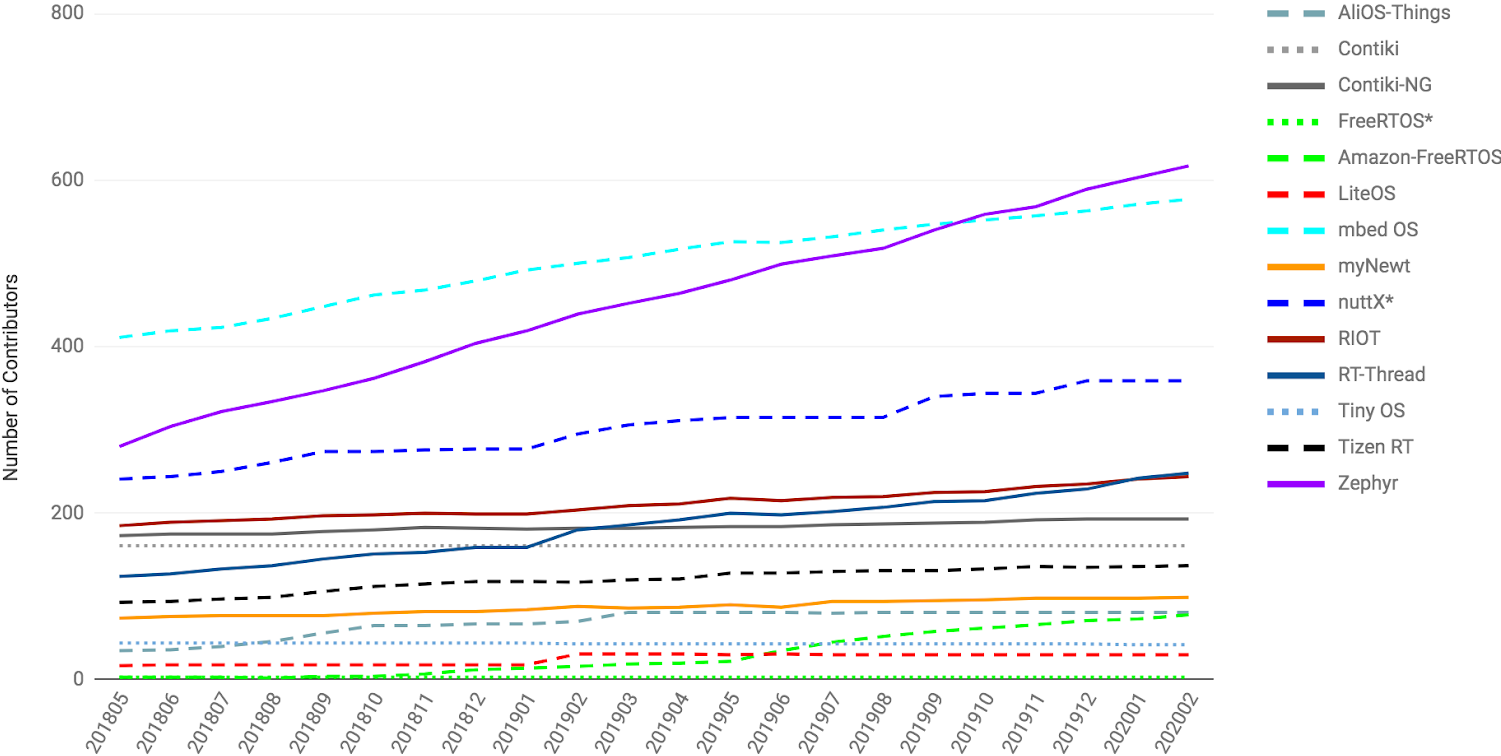
\includegraphics[width=4.5in]{apache.png}
\end{center}
 \caption{The trends in number of contributors across 14 real-time OS projects since 2018. Zephyr (one in purple) has 
  out-paced other similar software projects. (data source: The Apache Software Foundation)}\label{fig:apache}
 \end{figure} 
 
%  Since 2018 the
%   ZEPHYR real-time operating system has 
%   out-paced a dozen
%   other similar software projects (measured    in   contributors). Data from the Apache Foundation 
%   https://www.apache.org/. }\label{fig:apache}
%  \end{figure} 
 
\respto{4D} To give a scenario where this kind of prediction would be useful, we provide a real-world use case with a set of 14 real time OS projects currently supported by the Apache Software Foundation. As shown in Figure~\ref{fig:apache},  one of these operating systems, Zephyr (the one in purple), is exhibiting the steepest growth in the number of its contributors. As to the other projects, most
of these might be viewed as stagnant, perhaps even at risk of cancellation\footnote{In the Apache Software Foundation, projects can be canceled and  ``moved to the attic'' (https://attic.apache.org) when they are unable to muster 3 votes for a release, lack of active contributors, or unable to fulfill their reporting duties to the Foundation.}. 
Hence, to the managers of the stagnant
projects in Figure~\ref{fig:apache} (those with mostly flat curves),  they are particularly interested in ``catching up with  Zephyr''. Note that this
requires increasing
their number of contributors to the ``flat`` projects by 200\% (for RIOT) to 3,000\% (LiteOS). For that purpose,
predictions with a mere 19\% error (next month) would be useful
to foretell improvements to the software.


% (say) Knowledge about ``how many contributors in next month'' would help them making critical decisions for the project. With the existing data in Zephyr's development, DECART can be this kind of predicting tool. Based on Table~\ref{tbl:med_mre}, the median error rate of DECART is less than 20\% when predicting the number of contributors in the next month. Compared to some other commonly used analogy-based estimators (e.g. KNN, which has nearly 40\% error rate in this prediction)~\cite{shepperd1997estimating}, DECART improves the accuracy and provides useful prediction for those managers.
% Although it's not 100\% perfect, 


% Based on Table~\ref{tbl:med_mre}, the median error rate of DECART is less than 20\% when predicting the number of contributors in the next month. Suppose one of their projects will need 100 contributors next month, with the existing information in development, DECART can predict that less than 120 contributors are needed. Although this still suggests more personnel than needed, compared to some commonly used analogy-based estimations (e.g. KNN, which has nearly 40\% error rate in this prediction)~\cite{shepperd1997estimating}, 

 
 
%  XXX must double. XXXX our estimated only good to with 10\% but what the ehwllo. that would be enviguyht to show a if we are ront rack for the 200\% improvement needed to comete witht Zepht 


% (ZEPHYR\footnote{https://github.com/zephyrproject-rtos/zephyr})

% With the above experiment results, we can provide a real-world use case about how our methods can help for project planning in open source software development.  
% Recall the previous scenario we mentioned in the background, IBM developers need to know the expected workload within open-source toolkits they maintained in their software staff management~\cite{krishna2018connection}. Based on Table~\ref{tbl:med_mre}, the median error rate of DECART is less than 20\% when predicting the number of contributors in the next month. Suppose one of their projects will need 100 contributors next month, with the existing information in development, DECART can predict that less than 120 contributors are needed. Although this still suggests more personnel than needed, compared to some commonly used analogy-based estimations (e.g. KNN, which has nearly 40\% error rate in this prediction)~\cite{shepperd1997estimating}, it significantly improves the accuracy of personnel allocation, the costs of extra 20 contributors are saved for next month's staff management.
\BLACK







\subsection{What features matter the most in prediction? (RQ2)}
In our experimental data, we have 10 numeric features for prediction.
We use them since they are features with high importance, suggested by prior work (see Section~\ref{sect:data_collect}).
That said, having done all these experiments, it makes sense to ask which features, in practice, would be more useful when we predict health indicators.   This information could help us to focus on useful features and remove irrelevancies when enlarging our research in future work. To work that out, we look into the trees generated by DECART
(our best learners) in the above experiments. 
\BLUE
For each tree, we find impurity-based feature importances, which is computed as the normalized total reduction of the criterion brought by the feature (also known as the Gini importance). \respto{2D} \respto{4F}

For each predicting target, we calculate the mean scores for each feature, of all generated trees, the results are summarized in  Table~\ref{tbl:frq}. 
In this table, ``n/a''  denotes the dependent variable which is not counted in the experiment. From this table, first of all, we find that some features are highly related to specific health indicators. For example, ``commit'', ``openISSUE'' and  ``star'' have got scores  $23\%$,  $21\%$ and  $27\%$  when we built trees to predict ``contributor'' indicator for $1,159$ repositories.  Secondly, some features are bellwethers that have been used as features for multiple indicator predictions, like ``openPR'' gets $16\%$, $23\%$, $19\%$, and $26\%$ when predicting ``commit'', ``closePR'', ``openISSUE'' and ``closeISSUE''. Thirdly, some features even though they belong to the similar type, like ``openISSUE'' and ``closeISSUE'', they are not highly related in the predictions. In our experiment, we find that  ``openISSUE'' only gets $8\%$, way less than ``ISSUEcomment'' ($27\%$), ``openPR'' ($26\%$) and ``closePR'' ($13\%$) when predicting ``closeISSUE''. Last but not least,  some features are less used than others. According to our experiment, ``closePR'' is the least used feature for all predictions (the mean score of ``closePR'' is only 5\%).

\BLACK

\begin{blockquote}
\noindent
\textbf{Answer 2}: In our study, ``monthly\_commits'', ``monthly\_openPR'', ``monthly\_openISSUE'' and ``monthly\_closeISSUE'' are the most important features, while ``monthly\_closePR'' is the least used feature for all six health indicators' predictions.
\end{blockquote}

Note that none of these features should be abandoned. For feature ``closePR'', the least used feature in prediction, when predicting ``closeISSUE'', this feature still gets 13\% score of these cases.

 That said, it would be hard pressed to say
 that Table~\ref{tbl:frq} indicates that only a small subset of the \tbl{feature} features are outstandingly most important. While Table~\ref{tbl:frq} suggests that some feature pruning might be useful, overall we would suggest that using all of these features might be the best practice in most cases.


\begin{table*}[!b]
\centering

\begin{adjustbox}{max width=0.96\textwidth}
\begin{tabular}{r|cccccccccc}
\rowcolor[HTML]{FFFFFF}
{\color[HTML]{000000} Target } & \multicolumn{1}{l}{{\color[HTML]{000000} \begin{sideways}commit\end{sideways}}} & \multicolumn{1}{l}{{\color[HTML]{000000} \begin{sideways}contributor\end{sideways}}} & \multicolumn{1}{l}{{\color[HTML]{000000} \begin{sideways}openPR\end{sideways}}} & \multicolumn{1}{l}{{\color[HTML]{000000} \begin{sideways}closePR\end{sideways}}} & \multicolumn{1}{l}{{\color[HTML]{000000} \begin{sideways}openISSUE\end{sideways}}} & \multicolumn{1}{l}{{\color[HTML]{000000} \begin{sideways}closeISSUE\end{sideways}}} & \multicolumn{1}{l}{{\color[HTML]{000000} \begin{sideways}star\end{sideways}}} & \multicolumn{1}{l}{{\color[HTML]{000000} \begin{sideways}ISSUEcomment\end{sideways}}} & \multicolumn{1}{l}{{\color[HTML]{000000} \begin{sideways}mergedPR\end{sideways}}} & \multicolumn{1}{l}{{\color[HTML]{000000} \begin{sideways}fork\end{sideways}}} \\ \hline
\cellcolor[HTML]{FFFFFF}commit      & \cellcolor[HTML]{F4CCCC}n/a  & \cellcolor[HTML]{DEDEDE}5\%  & \cellcolor[HTML]{B3B3B3}16\% & \cellcolor[HTML]{EFEFEF}3\%  & \cellcolor[HTML]{DEDEDE}7\%  & \cellcolor[HTML]{A7A7A7}25\%                         & \cellcolor[HTML]{E7E7E7}4\%  & \cellcolor[HTML]{A5A5A5}21\% & \cellcolor[HTML]{DEDEDE}5\%  & \cellcolor[HTML]{B9B9B9}14\% \\
contributor & \cellcolor[HTML]{A3A3A3}23\% & \cellcolor[HTML]{F4CCCC}n/a  & \cellcolor[HTML]{CCCCCC}5\%  & \cellcolor[HTML]{DEDEDE}4\%  & \cellcolor[HTML]{A7A7A7}21\% & \cellcolor[HTML]{EFEFEF}3\%  & \cellcolor[HTML]{999999}27\% & \cellcolor[HTML]{CCCCCC}5\%  & \cellcolor[HTML]{C8C8C8}7\%  & \cellcolor[HTML]{CCCCCC}5\%  \\
openPR      & \cellcolor[HTML]{C8C8C8}9\%  & \cellcolor[HTML]{CCCCCC}7\%  & \cellcolor[HTML]{F4CCCC}n/a  & \cellcolor[HTML]{E2E2E2}4\%  & \cellcolor[HTML]{ABABAB}22\% & \cellcolor[HTML]{9C9C9C}30\%                         & \cellcolor[HTML]{EFEFEF}2\%  & \cellcolor[HTML]{DADADA}5\%  & \cellcolor[HTML]{B4B4B4}18\% & \cellcolor[HTML]{E9E9E9}3\%  \\
closePR     & \cellcolor[HTML]{B6B6B6}15\% & \cellcolor[HTML]{C3C3C3}11\% & \cellcolor[HTML]{9D9D9D}23\% & \cellcolor[HTML]{F4CCCC}n/a  & \cellcolor[HTML]{D3D3D3}8\%                          & \cellcolor[HTML]{A3A3A3}24\%                         & \cellcolor[HTML]{D3D3D3}7\%  & \cellcolor[HTML]{E1E1E1}5\%  & \cellcolor[HTML]{E8E8E8}4\%  & \cellcolor[HTML]{EFEFEF}3\%  \\
openISSUE   & \cellcolor[HTML]{EFEFEF}2\%  & \cellcolor[HTML]{E4E4E4}3\%  & \cellcolor[HTML]{A9A9A9}19\% & \cellcolor[HTML]{EFEFEF}2\%  & \cellcolor[HTML]{F4CCCC}n/a  & \cellcolor[HTML]{AEAEAE}17\% & \cellcolor[HTML]{CCCCCC}5\%  & \cellcolor[HTML]{D8D8D8}4\%  & \cellcolor[HTML]{999999}25\% & \cellcolor[HTML]{9F9F9F}23\% \\
closedISSUE & \cellcolor[HTML]{C7C7C7}10\% & \cellcolor[HTML]{EFEFEF}3\%  & \cellcolor[HTML]{9C9C9C}26\% & \cellcolor[HTML]{BFBFBF}13\% & \cellcolor[HTML]{DADADA}8\%                          & \cellcolor[HTML]{F4CCCC}n/a  & \cellcolor[HTML]{EFEFEF}3\%  & \cellcolor[HTML]{999999}27\% & \cellcolor[HTML]{DADADA}6\%  & \cellcolor[HTML]{E8E8E8}4\% \\ \hline
\rowcolor[HTML]{FFFFFF} 
mean & 12\% & 6\% & 18\% & 5\% & 13\% & 20\% & 8\% & 11\% & 11\% & 9\%
\end{tabular}
\end{adjustbox}
\caption{
The mean scores of Gini importance in trees generated by DECART (observed percentages in 1,159 cases).}
\label{tbl:frq}
\end{table*}

\subsection{Which methods achieve the best prediction performance? (RQ3)}
To answer this question, 
we compared the experimental results of each method on all 1,159 open-source projects predicting for 1, 3, 6, and 12 months into the future.  

\respto{2I}
\BLUE
Across 1,159 projects, we report the ``win rate'', which are the percentages of one learner belongs to the group with the best predictions performance (Rank=1). To get ``the group with the best prediction performance'', for each project, we use the Friedman test with Nemenyi Post-Hoc test introduced in Section~\ref{sect:stats} to compare different learners in terms of MRE and SA, then differentiate the learners into different groups, group with lower MRE (or larger SA) is the best group. One note is, there may be multiple methods belong to the best group (Rank=1). \tbl{win_mre} and \tbl{win_sa} show the results of learners' win rate in terms of MRE and SA.
\BLACK

The comparisons in these tables are for intra-row results, where the darker cells indicate the learning methods with higher win rate. For example, in the first row of \tbl{win_mre} (except the header row), when predicting the number of commits in next month, DECART has the best MRE performance in 74\% of all 1,159 cases. 

As shown in \tbl{win_mre}, in terms of MRE, DECART achieves the best performance with winning rates from $55\%$ to $91\%$ for all predictions (the median win rate is 76\%). 
\BLUE
Meanwhile, the winning rates of other learners, mostly range from $20\%$ to $60\%$. \respto{2A2} For example, FLASH, the hyperparameter-optimized method used in the previous effort estimation study, no longer works the best and its median win rate is only 59\%. 
In general, DECART outperforms other methods on almost all the predictions out of 1,159 projects by $10\% \sim 50\%$.
\BLACK

\begin{table}[!t]
\centering
\caption{MRE results: the win rate of different learners, measured in terms of MRE.}
\label{tbl:win_mre}
% \adjustbox{max width=.52\textwidth}{%
\resizebox{0.97\textwidth}{!}{
\begin{tabular}{llccccccccc}
\multicolumn{1}{c}{Predicting Month} & \multicolumn{1}{c}{Health Indicator} & KNN                          & LNR                          & SVR                          & RFT                          & CART                         & RDCART                       & GSCART                       & FLASH                        & DECART                       \\ \hline
                                     & commit                               & \cellcolor[HTML]{D2D2D2}42\% & \cellcolor[HTML]{F2F2F2}18\% & \cellcolor[HTML]{E7E7E7}26\% & \cellcolor[HTML]{D7D7D7}38\% & \cellcolor[HTML]{D6D6D6}39\% & \cellcolor[HTML]{CECECE}45\% & \cellcolor[HTML]{8F8F8F}74\% & \cellcolor[HTML]{ABABAB}61\% & \cellcolor[HTML]{8F8F8F}74\% \\
                                     & contributor                          & \cellcolor[HTML]{AEAEAE}60\% & \cellcolor[HTML]{E1E1E1}31\% & \cellcolor[HTML]{D1D1D1}43\% & \cellcolor[HTML]{CCCCCC}46\% & \cellcolor[HTML]{D4D4D4}41\% & \cellcolor[HTML]{CFCFCF}44\% & \cellcolor[HTML]{9E9E9E}67\% & \cellcolor[HTML]{B7B7B7}56\% & \cellcolor[HTML]{888888}77\% \\
                                     & openPR                               & \cellcolor[HTML]{CBCBCB}47\% & \cellcolor[HTML]{CDCDCD}46\% & \cellcolor[HTML]{DDDDDD}34\% & \cellcolor[HTML]{C6C6C6}49\% & \cellcolor[HTML]{BDBDBD}53\% & \cellcolor[HTML]{B4B4B4}57\% & \cellcolor[HTML]{8A8A8A}76\% & \cellcolor[HTML]{A9A9A9}62\% & \cellcolor[HTML]{6D6D6D}89\% \\
                                     & closePR                              & \cellcolor[HTML]{DDDDDD}34\% & \cellcolor[HTML]{E8E8E8}25\% & \cellcolor[HTML]{C2C2C2}51\% & \cellcolor[HTML]{C8C8C8}48\% & \cellcolor[HTML]{D0D0D0}43\% & \cellcolor[HTML]{D1D1D1}43\% & \cellcolor[HTML]{B9B9B9}55\% & \cellcolor[HTML]{B3B3B3}58\% & \cellcolor[HTML]{B6B6B6}56\% \\
                                     & openISSUE                            & \cellcolor[HTML]{C1C1C1}51\% & \cellcolor[HTML]{E5E5E5}28\% & \cellcolor[HTML]{EDEDED}22\% & \cellcolor[HTML]{D2D2D2}42\% & \cellcolor[HTML]{CDCDCD}46\% & \cellcolor[HTML]{C9C9C9}48\% & \cellcolor[HTML]{838383}79\% & \cellcolor[HTML]{A7A7A7}63\% & \cellcolor[HTML]{999999}69\% \\
\multirow{-6}{*}{1st month}          & closedISSUE                          & \cellcolor[HTML]{D3D3D3}41\% & \cellcolor[HTML]{E5E5E5}28\% & \cellcolor[HTML]{F1F1F1}19\% & \cellcolor[HTML]{D6D6D6}39\% & \cellcolor[HTML]{CFCFCF}44\% & \cellcolor[HTML]{CDCDCD}46\% & \cellcolor[HTML]{BBBBBB}54\% & \cellcolor[HTML]{CDCDCD}46\% & \cellcolor[HTML]{B9B9B9}55\% \\ \hline
                                     & commit                               & \cellcolor[HTML]{DADADA}36\% & \cellcolor[HTML]{E6E6E6}27\% & \cellcolor[HTML]{DEDEDE}33\% & \cellcolor[HTML]{CECECE}45\% & \cellcolor[HTML]{C9C9C9}48\% & \cellcolor[HTML]{CECECE}45\% & \cellcolor[HTML]{A7A7A7}63\% & \cellcolor[HTML]{ABABAB}61\% & \cellcolor[HTML]{898989}76\% \\
                                     & contributor                          & \cellcolor[HTML]{BFBFBF}52\% & \cellcolor[HTML]{E8E8E8}25\% & \cellcolor[HTML]{ECECEC}23\% & \cellcolor[HTML]{D4D4D4}41\% & \cellcolor[HTML]{DBDBDB}35\% & \cellcolor[HTML]{D7D7D7}38\% & \cellcolor[HTML]{767676}85\% & \cellcolor[HTML]{BBBBBB}54\% & \cellcolor[HTML]{696969}91\% \\
                                     & openPR                               & \cellcolor[HTML]{EAEAEA}24\% & \cellcolor[HTML]{D2D2D2}42\% & \cellcolor[HTML]{E1E1E1}31\% & \cellcolor[HTML]{D4D4D4}41\% & \cellcolor[HTML]{D3D3D3}41\% & \cellcolor[HTML]{CCCCCC}46\% & \cellcolor[HTML]{B9B9B9}55\% & \cellcolor[HTML]{B1B1B1}59\% & \cellcolor[HTML]{A0A0A0}66\% \\
                                     & closePR                              & \cellcolor[HTML]{DDDDDD}34\% & \cellcolor[HTML]{E9E9E9}25\% & \cellcolor[HTML]{D2D2D2}42\% & \cellcolor[HTML]{DADADA}36\% & \cellcolor[HTML]{B7B7B7}56\% & \cellcolor[HTML]{C4C4C4}50\% & \cellcolor[HTML]{8D8D8D}75\% & \cellcolor[HTML]{A5A5A5}64\% & \cellcolor[HTML]{989898}70\% \\
                                     & openISSUE                            & \cellcolor[HTML]{D5D5D5}40\% & \cellcolor[HTML]{EDEDED}22\% & \cellcolor[HTML]{E6E6E6}27\% & \cellcolor[HTML]{D0D0D0}43\% & \cellcolor[HTML]{D3D3D3}41\% & \cellcolor[HTML]{B3B3B3}58\% & \cellcolor[HTML]{A6A6A6}64\% & \cellcolor[HTML]{BBBBBB}54\% & \cellcolor[HTML]{ADADAD}60\% \\
\multirow{-6}{*}{3rd month}          & closedISSUE                          & \cellcolor[HTML]{DADADA}36\% & \cellcolor[HTML]{E6E6E6}27\% & \cellcolor[HTML]{E9E9E9}25\% & \cellcolor[HTML]{CFCFCF}44\% & \cellcolor[HTML]{D2D2D2}42\% & \cellcolor[HTML]{D1D1D1}43\% & \cellcolor[HTML]{666666}92\% & \cellcolor[HTML]{919191}73\% & \cellcolor[HTML]{777777}85\% \\ \hline
                                     & commit                               & \cellcolor[HTML]{D2D2D2}42\% & \cellcolor[HTML]{E7E7E7}26\% & \cellcolor[HTML]{E4E4E4}29\% & \cellcolor[HTML]{DADADA}36\% & \cellcolor[HTML]{C8C8C8}48\% & \cellcolor[HTML]{BFBFBF}52\% & \cellcolor[HTML]{888888}77\% & \cellcolor[HTML]{CECECE}45\% & \cellcolor[HTML]{6A6A6A}90\% \\
                                     & contributor                          & \cellcolor[HTML]{CDCDCD}46\% & \cellcolor[HTML]{DEDEDE}33\% & \cellcolor[HTML]{EDEDED}22\% & \cellcolor[HTML]{DEDEDE}33\% & \cellcolor[HTML]{C3C3C3}51\% & \cellcolor[HTML]{AEAEAE}60\% & \cellcolor[HTML]{B4B4B4}57\% & \cellcolor[HTML]{BEBEBE}52\% & \cellcolor[HTML]{9C9C9C}68\% \\
                                     & openPR                               & \cellcolor[HTML]{D3D3D3}41\% & \cellcolor[HTML]{DBDBDB}35\% & \cellcolor[HTML]{E2E2E2}30\% & \cellcolor[HTML]{D8D8D8}37\% & \cellcolor[HTML]{C7C7C7}48\% & \cellcolor[HTML]{C2C2C2}51\% & \cellcolor[HTML]{8A8A8A}76\% & \cellcolor[HTML]{B7B7B7}56\% & \cellcolor[HTML]{747474}86\% \\
                                     & closePR                              & \cellcolor[HTML]{E7E7E7}26\% & \cellcolor[HTML]{DFDFDF}32\% & \cellcolor[HTML]{DDDDDD}34\% & \cellcolor[HTML]{D4D4D4}41\% & \cellcolor[HTML]{CBCBCB}47\% & \cellcolor[HTML]{C4C4C4}50\% & \cellcolor[HTML]{919191}73\% & \cellcolor[HTML]{A3A3A3}65\% & \cellcolor[HTML]{ABABAB}61\% \\
                                     & openISSUE                            & \cellcolor[HTML]{CECECE}45\% & \cellcolor[HTML]{F1F1F1}19\% & \cellcolor[HTML]{E2E2E2}30\% & \cellcolor[HTML]{D7D7D7}38\% & \cellcolor[HTML]{CFCFCF}44\% & \cellcolor[HTML]{BDBDBD}53\% & \cellcolor[HTML]{A2A2A2}65\% & \cellcolor[HTML]{BDBDBD}53\% & \cellcolor[HTML]{8A8A8A}76\% \\
\multirow{-6}{*}{6th month}          & closedISSUE                          & \cellcolor[HTML]{CCCCCC}46\% & \cellcolor[HTML]{E4E4E4}28\% & \cellcolor[HTML]{EAEAEA}24\% & \cellcolor[HTML]{D7D7D7}38\% & \cellcolor[HTML]{CFCFCF}44\% & \cellcolor[HTML]{C8C8C8}48\% & \cellcolor[HTML]{BFBFBF}52\% & \cellcolor[HTML]{D1D1D1}43\% & \cellcolor[HTML]{A8A8A8}62\% \\ \hline
                                     & commit                               & \cellcolor[HTML]{CACACA}47\% & \cellcolor[HTML]{F3F3F3}17\% & \cellcolor[HTML]{E9E9E9}25\% & \cellcolor[HTML]{C4C4C4}50\% & \cellcolor[HTML]{DCDCDC}35\% & \cellcolor[HTML]{B1B1B1}58\% & \cellcolor[HTML]{9C9C9C}68\% & \cellcolor[HTML]{B6B6B6}56\% & \cellcolor[HTML]{818181}80\% \\
                                     & contributor                          & \cellcolor[HTML]{BABABA}55\% & \cellcolor[HTML]{EAEAEA}24\% & \cellcolor[HTML]{E0E0E0}31\% & \cellcolor[HTML]{DADADA}36\% & \cellcolor[HTML]{D9D9D9}37\% & \cellcolor[HTML]{BBBBBB}54\% & \cellcolor[HTML]{BABABA}55\% & \cellcolor[HTML]{AEAEAE}60\% & \cellcolor[HTML]{B5B5B5}57\% \\
                                     & openPR                               & \cellcolor[HTML]{D5D5D5}39\% & \cellcolor[HTML]{E5E5E5}28\% & \cellcolor[HTML]{E3E3E3}29\% & \cellcolor[HTML]{BFBFBF}52\% & \cellcolor[HTML]{BDBDBD}53\% & \cellcolor[HTML]{B9B9B9}55\% & \cellcolor[HTML]{7B7B7B}83\% & \cellcolor[HTML]{9A9A9A}69\% & \cellcolor[HTML]{6B6B6B}90\% \\
                                     & closePR                              & \cellcolor[HTML]{C7C7C7}49\% & \cellcolor[HTML]{EBEBEB}24\% & \cellcolor[HTML]{DADADA}36\% & \cellcolor[HTML]{D5D5D5}40\% & \cellcolor[HTML]{D3D3D3}41\% & \cellcolor[HTML]{CFCFCF}44\% & \cellcolor[HTML]{9E9E9E}67\% & \cellcolor[HTML]{A9A9A9}62\% & \cellcolor[HTML]{848484}79\% \\
                                     & openISSUE                            & \cellcolor[HTML]{C9C9C9}48\% & \cellcolor[HTML]{E6E6E6}27\% & \cellcolor[HTML]{E3E3E3}29\% & \cellcolor[HTML]{BEBEBE}53\% & \cellcolor[HTML]{CDCDCD}45\% & \cellcolor[HTML]{B9B9B9}55\% & \cellcolor[HTML]{C1C1C1}51\% & \cellcolor[HTML]{9E9E9E}67\% & \cellcolor[HTML]{808080}80\% \\
\multirow{-6}{*}{12th month}         & closedISSUE                          & \cellcolor[HTML]{DCDCDC}34\% & \cellcolor[HTML]{EBEBEB}23\% & \cellcolor[HTML]{EEEEEE}21\% & \cellcolor[HTML]{D9D9D9}37\% & \cellcolor[HTML]{D1D1D1}43\% & \cellcolor[HTML]{D1D1D1}43\% & \cellcolor[HTML]{696969}91\% & \cellcolor[HTML]{ABABAB}61\% & \cellcolor[HTML]{6D6D6D}89\% \\ \hline
                                     & \cellcolor[HTML]{FFFFFF}median       & \cellcolor[HTML]{FFFFFF}42\% & \cellcolor[HTML]{FFFFFF}27\% & \cellcolor[HTML]{FFFFFF}29\% & \cellcolor[HTML]{FFFFFF}41\% & \cellcolor[HTML]{FFFFFF}44\% & \cellcolor[HTML]{FFFFFF}49\% & \cellcolor[HTML]{FFFFFF}67\% & \cellcolor[HTML]{FFFFFF}59\% & \cellcolor[HTML]{FFFFFF}76\%
\end{tabular}
}
\end{table}


For SA results, as we see in \tbl{win_sa}, although the median win rate of DECART (69\%) decreased a bit compared to MRE (76\%), it still outperforms all the rest of methods (closest runner-up, GSCART gets 61\%). Specifically, DECAERT wins from $47\%$ to $84\%$ out of 4 different prediction ways on 1,159 projects. Compare to KNN wins from $21\%$ to $53\%$, LNR wins from $16\%$ to $43\%$, SVR wins from $19\%$ to $38\%$, RFT wins from $30\%$ to $56\%$, CART wins from $33\%$ to $56\%$, and tuned method RDCART wins from $41\%$ to $57\%$, GSCART wins from $47\%$ to $81\%$ and FLASH wins from $40\%$ to $75\%$, respectively. In most cases, the winning rates of the untuned methods  are less than $40\%$. After we take a further look, SVR performs relatively worse, the median winning rate is only $25\%$ compared to that of DECART, $69\%$. 



Based on the results from our experiments, we conclude that:
 

\begin{blockquote}
\noindent
\textbf{Answer 3}: 
DECART generates better prediction performance than other methods in 76\% of our 1,159 projects (MRE, median).
\end{blockquote}


\respto{2G4} \BLUE As state above, future work
might discover better optimizers
(for health indicator prediction) than DE. That said, these {\bf RQ3}
results tell us that DE   
 can find models that make better predictions  than many other approaches (that are used widely in the   literature). 
\BLACK





 



\section{Discussion}
\label{sect:discu}

% \BLUE
In this section, we look into the efficiency of our methods, and discuss the potential issues observed from experiment results.
\BLACK

\subsection{The efficiency of DECART}
 DECART   is not only effective (as shown in \tbl{win_mre} and \tbl{win_sa}), but also  very fast. In our study, it took around 4.3 hours to run DECART on 1,159 projects (on a dual-core 4.67 GHz desktop);
i.e. $13$ seconds per datasets. This time includes optimizing CART for each 
specific dataset, and then making predictions. Note that, for these experiments, we made no use of any special hardware (i.e. we used neither GPUs nor cloud services that interleave multiple cores in some clever manner).


The speed of DECART is an important finding. 
In our experience, the complexity of hyperparameter optimization is a major concern that limits its widespread use.   For example, Fu et al. report that hyperparameter optimization for
code defect prediction requires nearly three days of CPU per dataset~\cite{Fu2016TuningFS}.
If all of our 1,000+ datasets required the same amount of CPU resources, then it would be a major blocker to the use of the proposed methods in this paper.

But why is DECART so fast and effective?
Firstly,  DECART runs fast since it works on   very small datasets. 
This paper studies three to five years of project data. For each month, we  extract the 10 features shown in  Table~\ref{tbl:feature}. That is to say,  DECART's optimizations only have to explore datasets up to $\mathit{10*60}$
 data points per project.
  Fu et al. on the other hand, worked on more than 100,000 data points.
 
 
Secondly, as to why is DECART so effective, we note that many data mining algorithms  rely on  statistical properties that are emergent in   large samples of data~\cite{witten11}. Hence they  
have problems reasoning about  datasets with only $\mathit{10*60}$ data points.  
Accordingly, to enable effective data mining,
it is important to adjust the learners to the   idiosyncrasies of the dataset 
(via hyperparameter optimization).
 
\begin{table}[!t]
\centering
\caption{SA results:
the win rate of different learners, measured in terms of SA.}
\label{tbl:win_sa} 
% \adjustbox{max width=.52\textwidth}{%
\resizebox{0.97\textwidth}{!}{
\begin{tabular}{llccccccccc}
\multicolumn{1}{c}{Predicting Month} & \multicolumn{1}{c}{Health Indicator} & KNN                          & LNR                          & SVR                          & RFT                          & CART                         & RDCART                       & GSCART                       & FLASH                        & DECART                       \\ \hline
                                     & commit                               & \cellcolor[HTML]{D2D2D2}40\% & \cellcolor[HTML]{F2F2F2}18\% & \cellcolor[HTML]{E7E7E7}25\% & \cellcolor[HTML]{DCDCDC}33\% & \cellcolor[HTML]{D8D8D8}36\% & \cellcolor[HTML]{CECECE}43\% & \cellcolor[HTML]{767676}78\% & \cellcolor[HTML]{9C9C9C}63\% & \cellcolor[HTML]{8A8A8A}70\% \\
                                     & contributor                          & \cellcolor[HTML]{B5B5B5}53\% & \cellcolor[HTML]{D6D6D6}37\% & \cellcolor[HTML]{DCDCDC}33\% & \cellcolor[HTML]{CCCCCC}44\% & \cellcolor[HTML]{D9D9D9}35\% & \cellcolor[HTML]{D0D0D0}41\% & \cellcolor[HTML]{A6A6A6}59\% & \cellcolor[HTML]{B6B6B6}53\% & \cellcolor[HTML]{8A8A8A}70\% \\
                                     & openPR                               & \cellcolor[HTML]{C7C7C7}46\% & \cellcolor[HTML]{E9E9E9}24\% & \cellcolor[HTML]{DEDEDE}32\% & \cellcolor[HTML]{D0D0D0}42\% & \cellcolor[HTML]{BDBDBD}50\% & \cellcolor[HTML]{BBBBBB}51\% & \cellcolor[HTML]{838383}73\% & \cellcolor[HTML]{AFAFAF}56\% & \cellcolor[HTML]{8F8F8F}68\% \\
                                     & closePR                              & \cellcolor[HTML]{D9D9D9}35\% & \cellcolor[HTML]{DFDFDF}31\% & \cellcolor[HTML]{D5D5D5}38\% & \cellcolor[HTML]{CFCFCF}42\% & \cellcolor[HTML]{CDCDCD}44\% & \cellcolor[HTML]{C5C5C5}47\% & \cellcolor[HTML]{BBBBBB}51\% & \cellcolor[HTML]{AFAFAF}56\% & \cellcolor[HTML]{B8B8B8}52\% \\
                                     & openISSUE                            & \cellcolor[HTML]{CACACA}45\% & \cellcolor[HTML]{E8E8E8}25\% & \cellcolor[HTML]{F0F0F0}19\% & \cellcolor[HTML]{D6D6D6}37\% & \cellcolor[HTML]{CFCFCF}42\% & \cellcolor[HTML]{D0D0D0}42\% & \cellcolor[HTML]{777777}78\% & \cellcolor[HTML]{808080}74\% & \cellcolor[HTML]{8D8D8D}69\% \\
\multirow{-6}{*}{1st month}          & closedISSUE                          & \cellcolor[HTML]{D5D5D5}38\% & \cellcolor[HTML]{F0F0F0}19\% & \cellcolor[HTML]{EAEAEA}23\% & \cellcolor[HTML]{D7D7D7}37\% & \cellcolor[HTML]{D2D2D2}40\% & \cellcolor[HTML]{C9C9C9}45\% & \cellcolor[HTML]{C4C4C4}47\% & \cellcolor[HTML]{D2D2D2}40\% & \cellcolor[HTML]{BCBCBC}50\% \\ \hline
                                     & commit                               & \cellcolor[HTML]{DDDDDD}32\% & \cellcolor[HTML]{E9E9E9}24\% & \cellcolor[HTML]{DCDCDC}33\% & \cellcolor[HTML]{BDBDBD}50\% & \cellcolor[HTML]{CBCBCB}45\% & \cellcolor[HTML]{CCCCCC}44\% & \cellcolor[HTML]{AEAEAE}56\% & \cellcolor[HTML]{A2A2A2}61\% & \cellcolor[HTML]{828282}73\% \\
                                     & contributor                          & \cellcolor[HTML]{BEBEBE}50\% & \cellcolor[HTML]{EAEAEA}23\% & \cellcolor[HTML]{EDEDED}21\% & \cellcolor[HTML]{D8D8D8}36\% & \cellcolor[HTML]{D1D1D1}41\% & \cellcolor[HTML]{CACACA}45\% & \cellcolor[HTML]{747474}79\% & \cellcolor[HTML]{C6C6C6}47\% & \cellcolor[HTML]{929292}67\% \\
                                     & openPR                               & \cellcolor[HTML]{EEEEEE}21\% & \cellcolor[HTML]{E2E2E2}29\% & \cellcolor[HTML]{E7E7E7}25\% & \cellcolor[HTML]{D8D8D8}36\% & \cellcolor[HTML]{D3D3D3}40\% & \cellcolor[HTML]{C8C8C8}46\% & \cellcolor[HTML]{BBBBBB}51\% & \cellcolor[HTML]{AFAFAF}55\% & \cellcolor[HTML]{A3A3A3}60\% \\
                                     & closePR                              & \cellcolor[HTML]{DEDEDE}32\% & \cellcolor[HTML]{D4D4D4}39\% & \cellcolor[HTML]{D7D7D7}37\% & \cellcolor[HTML]{DCDCDC}33\% & \cellcolor[HTML]{AEAEAE}56\% & \cellcolor[HTML]{B6B6B6}53\% & \cellcolor[HTML]{8E8E8E}68\% & \cellcolor[HTML]{A0A0A0}61\% & \cellcolor[HTML]{808080}74\% \\
                                     & openISSUE                            & \cellcolor[HTML]{D9D9D9}35\% & \cellcolor[HTML]{CECECE}43\% & \cellcolor[HTML]{EAEAEA}23\% & \cellcolor[HTML]{D5D5D5}38\% & \cellcolor[HTML]{CACACA}45\% & \cellcolor[HTML]{C7C7C7}46\% & \cellcolor[HTML]{A7A7A7}59\% & \cellcolor[HTML]{C2C2C2}48\% & \cellcolor[HTML]{C5C5C5}47\% \\
\multirow{-6}{*}{3rd month}          & closedISSUE                          & \cellcolor[HTML]{DBDBDB}34\% & \cellcolor[HTML]{E9E9E9}24\% & \cellcolor[HTML]{EAEAEA}23\% & \cellcolor[HTML]{D0D0D0}41\% & \cellcolor[HTML]{D1D1D1}41\% & \cellcolor[HTML]{AEAEAE}56\% & \cellcolor[HTML]{737373}79\% & \cellcolor[HTML]{9D9D9D}63\% & \cellcolor[HTML]{666666}84\% \\ \hline
                                     & commit                               & \cellcolor[HTML]{D8D8D8}36\% & \cellcolor[HTML]{EBEBEB}22\% & \cellcolor[HTML]{EDEDED}21\% & \cellcolor[HTML]{DEDEDE}32\% & \cellcolor[HTML]{C6C6C6}46\% & \cellcolor[HTML]{C9C9C9}45\% & \cellcolor[HTML]{929292}67\% & \cellcolor[HTML]{B3B3B3}54\% & \cellcolor[HTML]{888888}71\% \\
                                     & contributor                          & \cellcolor[HTML]{C9C9C9}45\% & \cellcolor[HTML]{DEDEDE}31\% & \cellcolor[HTML]{DBDBDB}34\% & \cellcolor[HTML]{E0E0E0}30\% & \cellcolor[HTML]{C7C7C7}46\% & \cellcolor[HTML]{B9B9B9}52\% & \cellcolor[HTML]{B8B8B8}52\% & \cellcolor[HTML]{C9C9C9}45\% & \cellcolor[HTML]{A3A3A3}60\% \\
                                     & openPR                               & \cellcolor[HTML]{D3D3D3}40\% & \cellcolor[HTML]{D1D1D1}41\% & \cellcolor[HTML]{E4E4E4}28\% & \cellcolor[HTML]{D7D7D7}37\% & \cellcolor[HTML]{C4C4C4}47\% & \cellcolor[HTML]{C7C7C7}46\% & \cellcolor[HTML]{8C8C8C}69\% & \cellcolor[HTML]{B5B5B5}53\% & \cellcolor[HTML]{696969}83\% \\
                                     & closePR                              & \cellcolor[HTML]{E6E6E6}26\% & \cellcolor[HTML]{E1E1E1}29\% & \cellcolor[HTML]{E2E2E2}29\% & \cellcolor[HTML]{DADADA}35\% & \cellcolor[HTML]{D2D2D2}40\% & \cellcolor[HTML]{B6B6B6}53\% & \cellcolor[HTML]{717171}80\% & \cellcolor[HTML]{979797}65\% & \cellcolor[HTML]{737373}79\% \\
                                     & openISSUE                            & \cellcolor[HTML]{D1D1D1}41\% & \cellcolor[HTML]{F0F0F0}19\% & \cellcolor[HTML]{ECECEC}22\% & \cellcolor[HTML]{D7D7D7}36\% & \cellcolor[HTML]{D2D2D2}40\% & \cellcolor[HTML]{B9B9B9}52\% & \cellcolor[HTML]{ACACAC}57\% & \cellcolor[HTML]{BCBCBC}50\% & \cellcolor[HTML]{8F8F8F}68\% \\
\multirow{-6}{*}{6th month}          & closedISSUE                          & \cellcolor[HTML]{D9D9D9}35\% & \cellcolor[HTML]{E7E7E7}25\% & \cellcolor[HTML]{E9E9E9}24\% & \cellcolor[HTML]{DCDCDC}33\% & \cellcolor[HTML]{D1D1D1}41\% & \cellcolor[HTML]{CDCDCD}44\% & \cellcolor[HTML]{BFBFBF}49\% & \cellcolor[HTML]{CDCDCD}44\% & \cellcolor[HTML]{B3B3B3}54\% \\ \hline
                                     & commit                               & \cellcolor[HTML]{CDCDCD}44\% & \cellcolor[HTML]{F3F3F3}16\% & \cellcolor[HTML]{F0F0F0}19\% & \cellcolor[HTML]{C3C3C3}48\% & \cellcolor[HTML]{DDDDDD}33\% & \cellcolor[HTML]{ADADAD}57\% & \cellcolor[HTML]{A8A8A8}58\% & \cellcolor[HTML]{B0B0B0}55\% & \cellcolor[HTML]{8D8D8D}69\% \\
                                     & contributor                          & \cellcolor[HTML]{B2B2B2}54\% & \cellcolor[HTML]{EBEBEB}22\% & \cellcolor[HTML]{E5E5E5}27\% & \cellcolor[HTML]{D8D8D8}36\% & \cellcolor[HTML]{D9D9D9}35\% & \cellcolor[HTML]{C6C6C6}47\% & \cellcolor[HTML]{BBBBBB}51\% & \cellcolor[HTML]{A8A8A8}58\% & \cellcolor[HTML]{AEAEAE}56\% \\
                                     & openPR                               & \cellcolor[HTML]{D9D9D9}36\% & \cellcolor[HTML]{E3E3E3}28\% & \cellcolor[HTML]{E5E5E5}27\% & \cellcolor[HTML]{BFBFBF}49\% & \cellcolor[HTML]{C2C2C2}48\% & \cellcolor[HTML]{ABABAB}57\% & \cellcolor[HTML]{6F6F6F}81\% & \cellcolor[HTML]{7D7D7D}75\% & \cellcolor[HTML]{9C9C9C}63\% \\
                                     & closePR                              & \cellcolor[HTML]{C3C3C3}48\% & \cellcolor[HTML]{E7E7E7}25\% & \cellcolor[HTML]{DEDEDE}31\% & \cellcolor[HTML]{D7D7D7}37\% & \cellcolor[HTML]{D6D6D6}37\% & \cellcolor[HTML]{D2D2D2}40\% & \cellcolor[HTML]{A7A7A7}59\% & \cellcolor[HTML]{ACACAC}57\% & \cellcolor[HTML]{929292}67\% \\
                                     & openISSUE                            & \cellcolor[HTML]{D1D1D1}41\% & \cellcolor[HTML]{DFDFDF}31\% & \cellcolor[HTML]{E7E7E7}25\% & \cellcolor[HTML]{AEAEAE}56\% & \cellcolor[HTML]{CDCDCD}44\% & \cellcolor[HTML]{B6B6B6}53\% & \cellcolor[HTML]{7B7B7B}76\% & \cellcolor[HTML]{A4A4A4}60\% & \cellcolor[HTML]{818181}74\% \\
\multirow{-6}{*}{12th month}         & closedISSUE                          & \cellcolor[HTML]{DCDCDC}33\% & \cellcolor[HTML]{E0E0E0}30\% & \cellcolor[HTML]{ECECEC}22\% & \cellcolor[HTML]{DADADA}35\% & \cellcolor[HTML]{D4D4D4}38\% & \cellcolor[HTML]{CFCFCF}42\% & \cellcolor[HTML]{9F9F9F}62\% & \cellcolor[HTML]{AFAFAF}56\% & \cellcolor[HTML]{7D7D7D}75\% \\ \hline
                                     & median                               & 39\%                         & 25\%                         & 25\%                         & 37\%                         & 41\%                         & 46\%                         & 61\%                         & 56\%                         & 69\%                        
\end{tabular}
 }
\end{table} 



\subsection{DECART on other time predictions}
\label{sect:other}
In our experiment, we observe that when predicting specific health indicators, DECART can achieve 0\% error in some cases. Such zero error is a red flag that needs to be investigated since they might be due to overfitting or programming errors (such as use the test value as both the predicted and actual value for the MRE calculation). What we found was that the older the project, the less the programmer activity.
  Hence,  it is hardly surprising that good learners could correctly predict (e.g.) zero closed pull requests.


But that raises another red flag: suppose {\em all} our projects had reached some steady state prior to April 2020. In that case, predicting (say) the next month's value of health indicator would be a simple matter of repeating last month's value. In our investigation, we have three reasons for believing that this is not the case.
Firstly, prediction in this domain is difficult. If such steady state had been achieved, then all our learners would be reporting very low errors. As seen in Table~\ref{tbl:med_mre}, this is not the case.

Secondly, we looked into the columns in our raw data, looking for long sequences of stable or zero values. This case does not happen in most cases: our data contains many variations across the entire lifecycle of our projects.

Thirdly, just to be sure, we conducted another round of experiments. Instead of predicting for the most recent months, we do the prediction for an earlier period using
data collected prior to that time point.
Table~\ref{tbl:mid} shows the results. In this table, if a project had (say) $N=60$ months of data, we went to months $N/2$ and used DECART to predicted 12 months into the future (to $N/2+12$). The columns for Table~\ref{tbl:mid}  should be compared to the right-hand-side columns of Table~\ref{tbl:med_mre}, Table~\ref{tbl:iqr_mre},  Table~\ref{tbl:med_sa}, and Table~\ref{tbl:iqr_sa}. In that comparison, we see that predicting for months in mid period can
generate comparable results as predicting for most recent months.
 
In summary, our results are not unduly biased by predicting just for the recent months. As the evidence, we can still obtain accurate results if we predict for earlier months.


\begin{table}[!b]
\centering

\begin{adjustbox}{max width=0.98\textwidth}
\begin{tabular}{lrrrr}
            & \multicolumn{1}{c}{Median MRE} & \multicolumn{1}{c}{IQR MRE}   & \multicolumn{1}{c}{Median SA} & \multicolumn{1}{c}{IQR SA}    \\
commit      & \cellcolor[HTML]{F3F3F3}67\%   & \cellcolor[HTML]{F3F3F3}124\% & \cellcolor[HTML]{F3F3F3}29\%  & \cellcolor[HTML]{F3F3F3}112\% \\
contributor & \cellcolor[HTML]{FFFFFF}44\%   & \cellcolor[HTML]{FFFFFF}83\%  & \cellcolor[HTML]{FFFFFF}40\%  & \cellcolor[HTML]{FFFFFF}133\% \\
openPR      & \cellcolor[HTML]{F3F3F3}38\%   & \cellcolor[HTML]{F3F3F3}77\%  & \cellcolor[HTML]{F3F3F3}37\%  & \cellcolor[HTML]{F3F3F3}106\% \\
closePR     & \cellcolor[HTML]{FFFFFF}64\%   & \cellcolor[HTML]{FFFFFF}104\% & \cellcolor[HTML]{FFFFFF}27\%  & \cellcolor[HTML]{FFFFFF}87\%  \\
openISSUE   & \cellcolor[HTML]{F3F3F3}52\%   & \cellcolor[HTML]{F3F3F3}73\%  & \cellcolor[HTML]{F3F3F3}29\%  & \cellcolor[HTML]{F3F3F3}164\% \\
closedISSUE & \cellcolor[HTML]{FFFFFF}37\%   & \cellcolor[HTML]{FFFFFF}68\%  & \cellcolor[HTML]{FFFFFF}34\%  & \cellcolor[HTML]{FFFFFF}116\%
\end{tabular}
\end{adjustbox}
\caption{The performance of DECART, staring mid-way through a project, then predicting 12 months into the future.}
\label{tbl:mid}
\end{table}


\section{Threats to validity}
\label{sect:threa}
The design of this study may have several validity threats~\cite{feldt2010validity}. The following issues should be considered to avoid jeopardizing conclusions made from this work.
 

\textbf{Parameter Bias:} The settings to control the hyperparameters of the prediction methods can have a positive effect on the efficacy of the prediction. By using hyperparameter optimized method in our experiment, we explore the space of possible hyperparameters for the predictor, hence we assert that this study suffers less parameter bias than some other studies.

\BLUE
\textbf{Survey Bias:} \respto{4B2} To verify whether our potential health indicators actually matter, we made a survey to open source project developers to ask about their opinions based on their development experience. While most features were considered to be relevant to the project health in the survey, we would not claim the result was a complete set of project health indicators. In our survey, the choice of features was limited to several options in order to keep it easy to respond. Although the participants could provide additional thoughts in the following question, this would still narrow down their opinions. In future, additional knowledge from participants will be added to reduce this bias. 
\BLACK

\textbf{Metric Bias:} We use Magnitude of the Relative Error (MRE) as one of the performance metrics in the experiment. However, MRE is criticized because of its bias towards error underestimations~\cite{foss2003simulation,kitchenham2001accuracy,korte2008confidence,port2008comparative,shepperd2000building,stensrud2003further}. Specifically, when the benchmark error is small or equal to zero, the relative error could become extremely large or infinite. This may lead to an undefined mean or at least a distortion of the result~\cite{chen2017new}. In our study, we do not abandon MRE since there exist known baselines for human performance in effort estimation expressed in terms of MRE~\cite{Jorgensen03}. To overcome this limitation, we set a customized MRE treatment to deal with ``divide by zero'' issue and also apply Standardized Accuracy (SA) as the other measure of the performance.

\textbf{Sampling Bias:} 
In our study, we collect 64,181 months with 12 features of 1,159 GitHub projects data for the experiment, and use 6 GitHub development features as health indicators of open-source project. While we reach good prediction performance on those data, it would be inappropriate to conclude that our technique always gets positive result on open-source projects, or the health indicators we use could completely decide the project's health status. 
Another confounding factor is, since the projects we collected have different sizes, domains, life-cycles, etc., they could have different factors regarding the predicting performance of health indicators.
\BLUE
\respto{4G2} 
Also, in the study, we focus on the active project for the data collection. Those excluded inactive repositories might also provide useful data about how projects failed then give more exemplars for model training.
\BLACK
To mitigate these problems, we release open source resources of our work to support the research community to reproduce, improve or refute our results on broader data and indicators.

 

% \section{Other Related work}
% \label{sect:related}

% Our experiment data of open source project come from GitHub. As the largest and the most popular open source software development platform, GitHub hosts thousands of open source projects in different domains. When developing projects on GitHub, developers use fork to create their own copies of repositories, and submit pull requests when they want project maintainers to merge their commits into main branch~\cite{kalliamvakou2016depth}. People having questions can create issue on projects to notice developers. Also, if community members are interested in projects, they can add star to them.

% For software engineering studies, many techniques and suggestions are used to collect data from GitHub. Gousios et al. porpose a system named ``GHTorrent'' which creates a scalable, queriable, offline mirror of data offered through the GitHub REST API~\cite{gousios2012ghtorrent}, this work offers great resources to the research community because of its various and enormous amount of data. As a following work, they also provide a dataset for Pull-Based development research which contains 350,000 pull requests from almost 900 GitHub projects~\cite{gousios2014dataset}. 

% The quantity of open source research data would no longer to be in severe shortage. However, not every repository on GitHub is useful for research purposes.
% Munaiah et al. indicate that many GitHub repositories are ``noise''
% (e.g. home work assignments) which may not be appropriate for research purposes~\cite{munaiah2017curating}. They porpose a tool named ``reaper'' which uses score-based classifiers and random forest to help researchers finding GitHub repositories that contain engineered software projects.

% Some GitHub projects tend to be no longer active anymore. Coelho et al. collect a set of project activity features (e.g. commits, forks, issues, etc), and train random forest based models to help detecting those GitHub projects which lack of maintenance, and alert potential users about the risks of using these projects~\cite{coelho2018identifying}.

% Also, Kalliamvakou et al. conduct a study about understanding the characteristics of the repositories in GitHub and how users take advantage of GitHub’s main features. They find that mining GitHub for research purposes could take various potential perils and provide a set of recommendations for software engineering researchers on mining data from GitHub~\cite{kalliamvakou2014promises,kalliamvakou2016depth}.


\section{Conclusion and Future Work}
\label{sect:concl}

 

Our results make a compelling case for open source software projects. 
% Companies that only build in-house proprietary products may be cutting themselves off from the information needed to reason about those projects. 
Software developed on some public platforms is a source of data that can be used to make accurate predictions  about those projects. While the activity of a single developer may be random and hard to predict, when large groups of developers work together on software projects,
the resulting behavior can be predicted with good accuracy. For example, after building predictors for six project health indicators, we can make predictions with low error rates (median values usually under 25\%). 

\BLUE
Our results come with some caveats. The patterns of some activities are harder to be learned, for the law of large numbers. We know this since we cannot constantly get high accuracy in predictions. For example, 
across our six health indicators, the predicting performances of closePR and commit are not as good as when predicting the number of contributors (as shown in Table~\ref{tbl:med_mre}). 
\BLACK
 Also, to make predictions, we must take care to tune the data mining algorithms to the idiosyncrasies of the datasets.
 Some data mining algorithms rely on statistical properties that are emergent in large samples of data.
 Hence, such algorithms may have problems reasoning about very small datasets, such as those studied here.
 Hence, before making predictions, it is vitally   important to adjust the learners to the idiosyncrasies of the dataset via hyperparameter optimization. Unlike prior hyperparameter optimization work by Fu et al.~\cite{Fu2016TuningFS}, our optimization process is very fast (a few seconds per dataset). Accordingly, we assert that for predicting project health indicators, hyperparameter optimization is the preferred technology.
 
As to future work, there is still much to do. 
Firstly, we know many organizations such as IBM that run large in-house ecosystems where, behind firewalls, thousands of programmers build software using  a private GitHub system. It would be insightful to see if our techniques work for such ``private'' GitHub networks.
\BLUE
\respto{2G5} \respto{4H1} Secondly, our results still have large space to improve. Some prediction tasks are harder than others
(e.g. commits, closed PR).
% The DE algorithm used in this paper is essentially Storn's 1997 version and there are many more recent variants of that algorithm that could be useful. 
In our study, DE has shown good prediction performance comparing to other methods, exploring other evolutionary algorithms~\cite{wu2018ensemble,das2016recent} on different learners (e.g. random forest) or applying auto-sklearn~\cite{feurer2019auto} could be useful and might bring even better results.

Further, as to more indicators, there are more practices from real-world business-level cases to explore. 
\respto{4B3}
In our survey, some of the participants mentioned other features they think are relevant to open source project health, we will assess their opinions to find more indicators. 
\respto{4I2} 
Also, it would be worth trying if we can derive more effective sophisticated health indicators, such as:

\bi
\item
The number of new joining/leaving contributors.
\item
The change in number of developing features (commits, contributors, openPR, etc.) over time.
\ei

\respto{4G3} 
Lastly, an enriched data collection with more features from more types of repositories (e.g. inactive or archived projects) would be helpful for our model learning. With enough training data, we could also explore deep neural network methods (e.g. LSTM) on projects from thousands of repositories, and try to detect anomalies in their developments that may jeopardize the health of these software projects.
\BLACK


\section*{Acknowledgements}
This work is partially funded by a National Science Foundation
Grant \#1703487.

%%
%% The next two lines define the bibliography style to be used, and
%% the bibliography file.
% \newpage 
% \balance
\bibliographystyle{ACM-Reference-Format}
\bibliography{bibreference}



\end{document}
\endinput
%%
%% End of file `sample-sigchi.tex'.
